%%%%%%%%%%%%%%%%%%%%% {{{
%%Options for presentations (in-class) and handouts (e.g. print).
% \documentclass[pdf,9pt]{beamer}
\documentclass[pdf,9pt]{beamer}


%%%%%%%%%%%%%%%%%%%%%%
%Change this for different slides so it appears in bar
\usepackage{authoraftertitle}
\date{Chapter 8. Orthogonality \\ \S  8-6. Singular Value Decomposition}

%%%%%%%%%%%%%%%%%%%%%%
%% Upload common style file
\usepackage{LyryxLAWASlidesStyle}

\begin{document}

%%%%%%%%%%%%%%%%%%%%%%%
%% Title Page and Copyright Common to All Slides

%Title Page
\input frontmatter/titlepage.tex

%LOTS Page
\input frontmatter/lyryxopentexts.tex

%Copyright Page
\input frontmatter/copyright.tex

%%%%%%%%%%%%%%%%%%%%%%%%% }}}
%-------------- start slide -------------------------------%{{{ 2

\begin{frame}[fragile]
   \tableofcontents
\end{frame}
%-------------- end slide -------------------------------%}}}
\section[\textcolor{yellow}{}]{\textcolor{yellow}{Singular Value Decomposition}}
%-------------- start slide -----------------------------% {{{ 3
\frame{
\frametitle{Singular Value Decomposition}
\pause
\begin{center}
    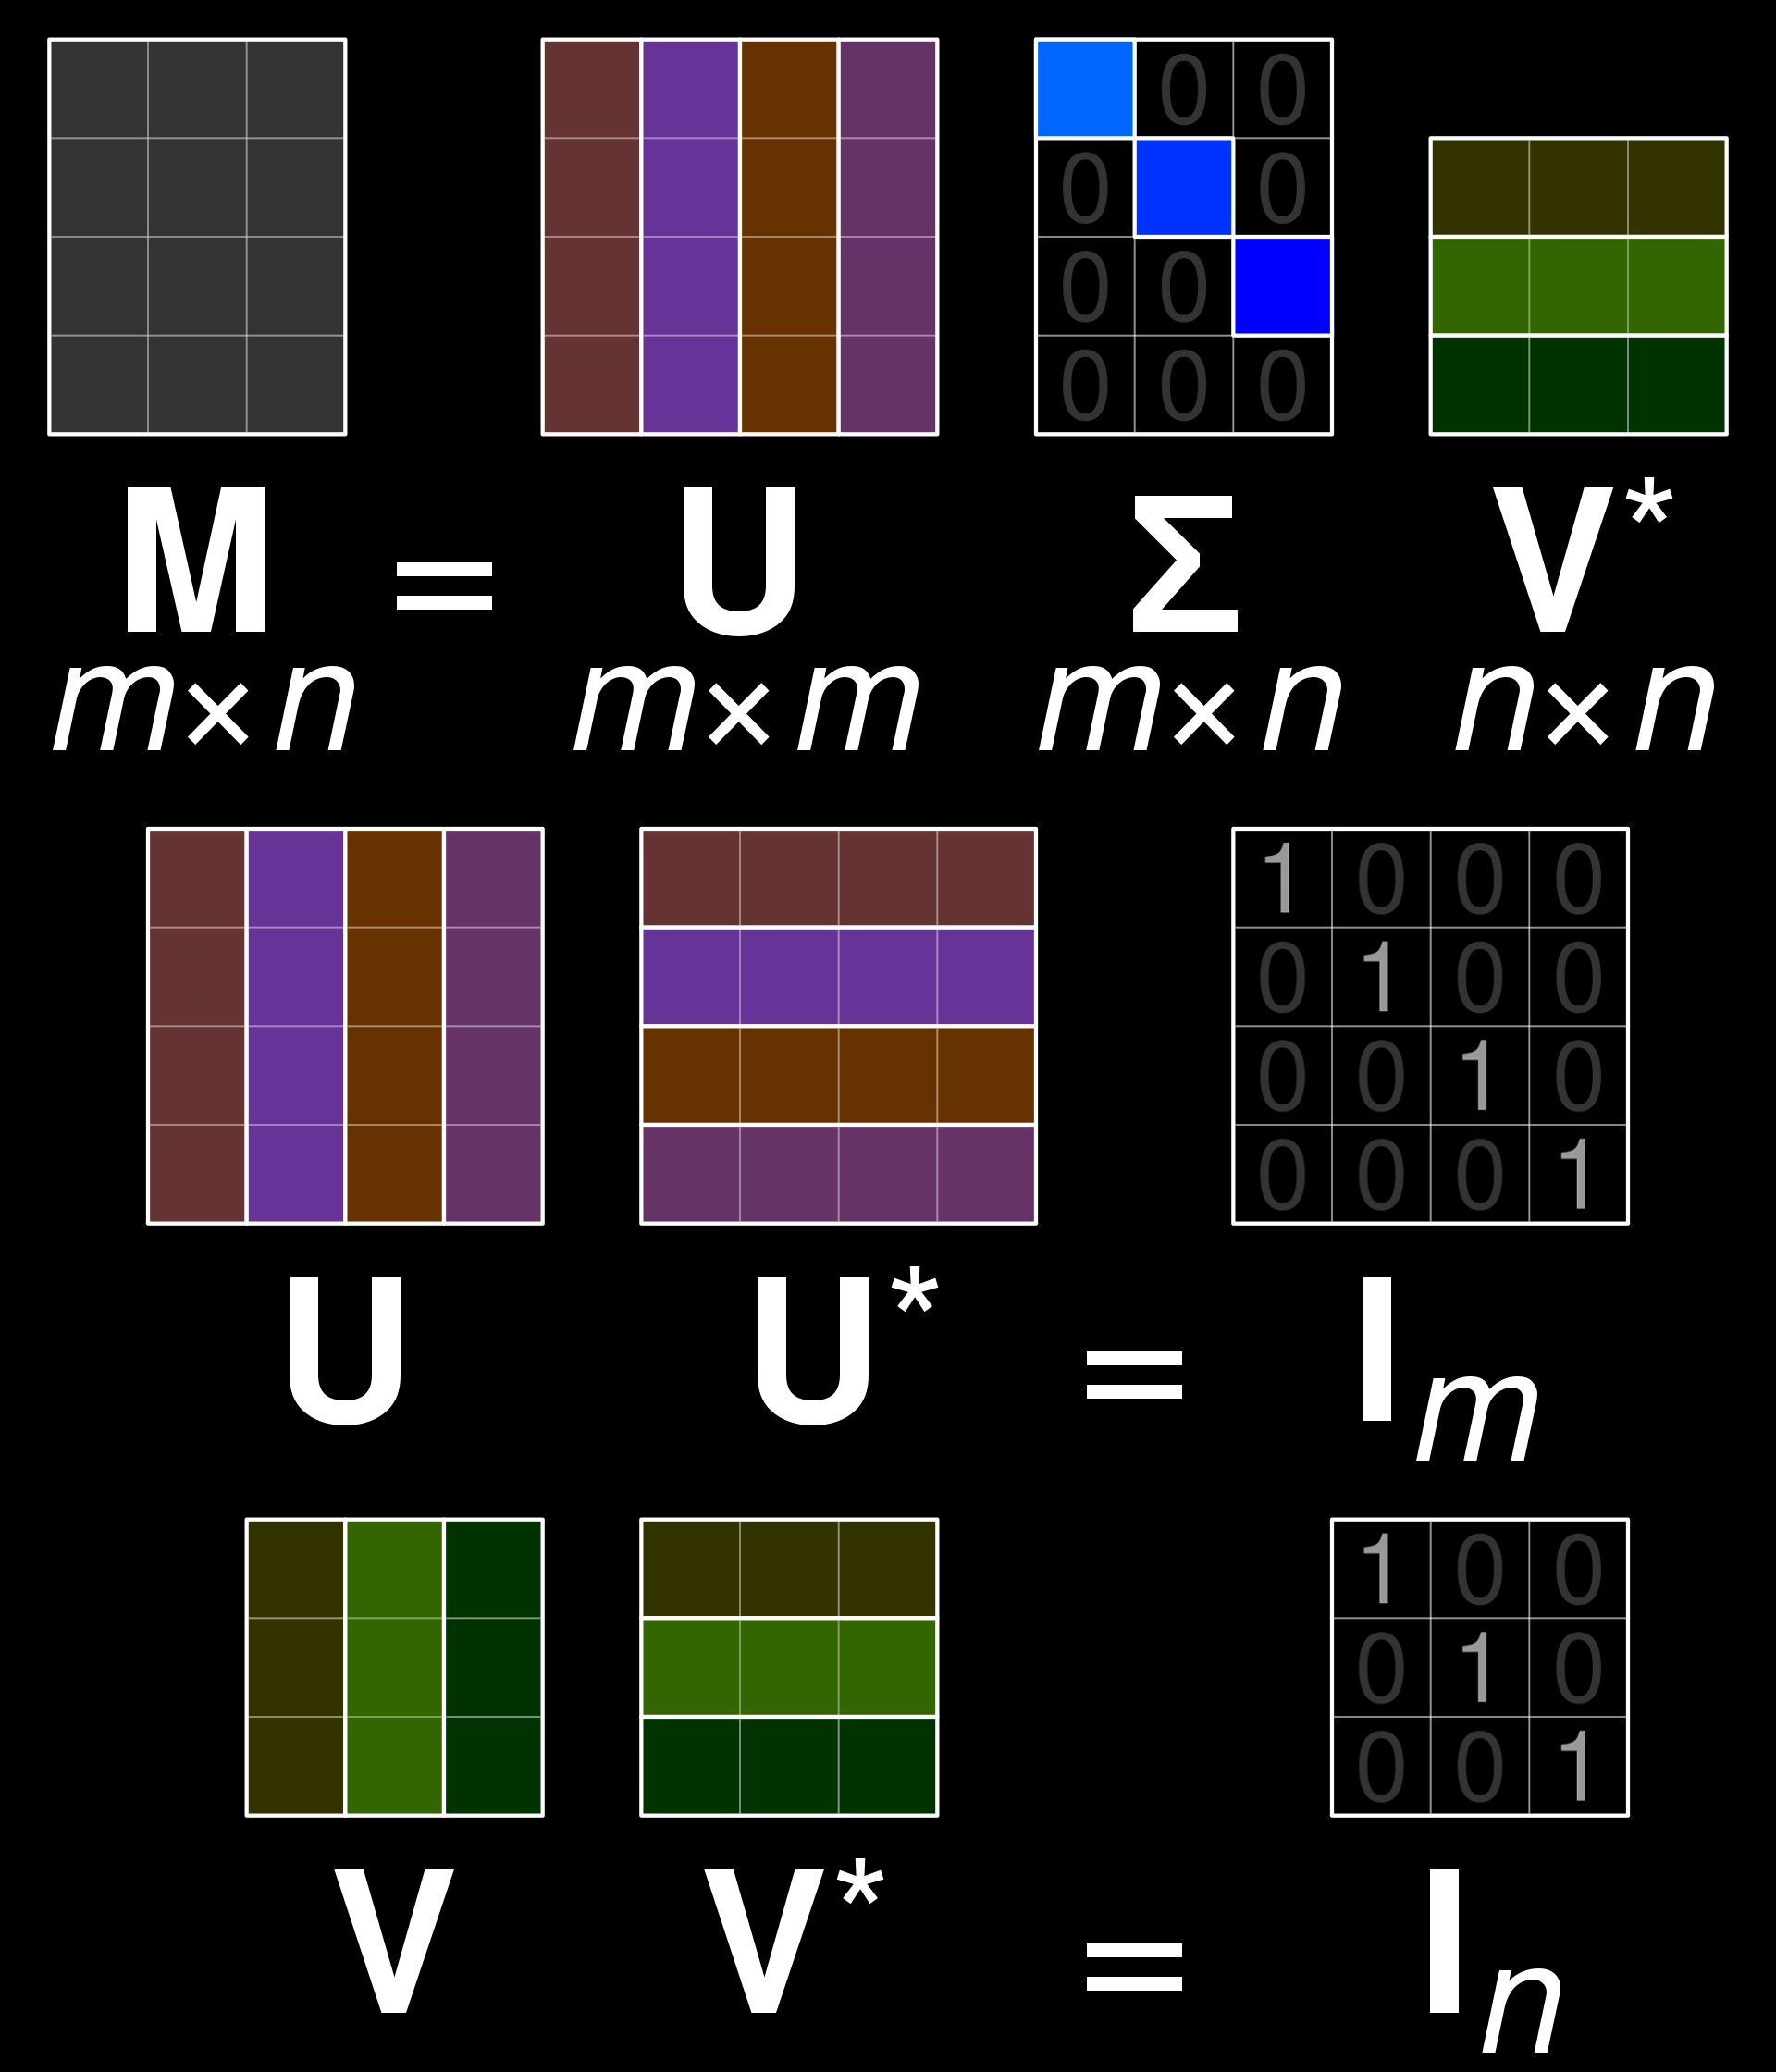
\includegraphics[scale=0.06]{./figures/SVD-neg.png}
\end{center}
}
%-------------- end slide -------------------------------%}}}
%-------------- start slide -----------------------------% {{{ 4
\frame{
\begin{definition}
    Let $A$ be an $m\times n$ matrix.
    The \alert{singular values} of $A$ are the square roots of the nonzero
    eigenvalues of $A^TA$.
    \pause
    \alert{Singular Value Decomposition (SVD)} can be thought of as
    a generalization of orthogonal diagonalization of a symmetric matrix
    to an arbitrary $m\times n$ matrix.
    \pause

    Given an $m\times n$ matrix $A$, we will see how to express $A$ as
    a product
    \[ A=U\Sigma V^T\]
    where
    \bigskip
    \pause
    \begin{itemize}
	\item $U$ is an $m\times m$ orthogonal matrix whose columns are eigenvectors of $AA^T$.
	    \pause
	    \bigskip
	\item $V$ is an $n\times n$ orthogonal matrix whose columns are eigenvectors of $A^TA$.
	    \pause
	    \bigskip
	\item $\Sigma$ is an $m\times n$ matrix whose only nonzero values
	    lie on its main diagonal, and are the square roots of the eigenvalues
	    of both $AA^T$ and $A^TA$.
    \end{itemize}
\end{definition}
}
%-------------- end slide -------------------------------%}}}
%-------------- start slide -----------------------------% {{{ 5
\frame{
\begin{theorem}
    If $A$ is an $m\times n$ matrix, then $A^TA$ and $AA^T$ have the same nonzero eigenvalues.
\end{theorem}
\pause
\vfill
\begin{proofnoend}
    Suppose $A$ is an $m\times n$ matrix, and suppose that
    $\lambda$ is a nonzero eigenvalue of $A^TA$.
    Then there exists a nonzero vector $\vec{x}\in \RR^n$ such that
    % \vspace*{-.02in}

    \begin{equation}\label{nonzero}
	(A^TA)\vec{x}=\lambda \vec{x}.
    \end{equation}

    Multiplying both sides of this equation by $A$:
    \begin{eqnarray*}
	A(A^TA)\vec{x}   & = & A\lambda \vec{x} \\
	(AA^T)(A\vec{x}) & = & \lambda (A\vec{x}).
    \end{eqnarray*}
    Since $\lambda\neq 0$ and $\vec{x}\neq \vec{0}_n$,
    $\lambda \vec{x}\neq\vec{0}_n$,
    and thus by equation~(\ref{nonzero}),
    $(A^TA)\vec{x}\neq\vec{0}_n$; thus $A^T(A\vec{x})\neq\vec{0}_n$,
    implying that $A\vec{x}\neq\vec{0}_m$.
    \medskip

    Therefore $A\vec{x}$ is an eigenvector of $AA^T$ corresponding
    to eigenvalue $\lambda$.
    An analogous argument can be used to show that every nonzero
    eigenvalue of $AA^T$ is an eigenvalue of $A^TA$, thus completing
    the proof.
    \myQED
\end{proofnoend}
}
%-------------- end slide -------------------------------%}}}
\section[\textcolor{yellow}{}]{\textcolor{yellow}{Examples}}
%-------------- start slide -----------------------------% {{{{ 6
\frame{
\frametitle{Examples}
\pause
\begin{example}
    Let
    $A=\left[\begin{array}{rrr} 1 & -1 & 3 \\ 3 & 1 & 1 \end{array}\right]$.
    Then
    \[ AA^T =
	\left[\begin{array}{rrr} 1 & -1 & 3 \\ 3 & 1 & 1 \end{array}\right]
	\left[\begin{array}{rr} 1 & 3 \\ -1 & 1 \\ 3 & 1  \end{array}\right] =
	\left[\begin{array}{rr} 11 & 5 \\ 5 & 11  \end{array}\right].\]
    \[ A^TA =
	\left[\begin{array}{rr}  1 & 3  \\ -1 &  1 \\ 3 & 1 \end{array}\right]
	\left[\begin{array}{rrr} 1 & -1 &  3  \\ 3 &  1 & 1 \end{array}\right] =
	\left[\begin{array}{rrr} 10 & 2 & 6 \\ 2 & 2 & -2\\ 6 & -2 & 10 \end{array}\right].\]
\end{example}
}
%-------------- end slide -------------------------------%}}}
%-------------- start slide -------------------------------%{{{{ 7
\begin{frame}[fragile]
\begin{example}[continued]
Since $AA^T$ is $2\times 2$ while $A^T A$ is $3\times 3$, and
$AA^T$ and $A^TA$ have the same {\em nonzero} eigenvalues, compute
$c_{AA^T}(x)$ (because it's easier to compute than $c_{A^TA}(x)$).

% \vspace*{-.2in}
\begin{eqnarray*}
    c_{AA^T}(x) & = & \det(xI-AA^T)= \left|\begin{array}{cc} x-11  & -5 \\ -5 & x-11 \end{array}\right| \\
                & = & (x-11)^2 - 25                               \\
                & = & x^2-22x+121-25                              \\
                & = & x^2-22x+96                                  \\
                & = & (x-16)(x-6).
\end{eqnarray*}

% \vspace*{-.05in}
Therefore, the eigenvalues of $AA^T$ are $\lambda_1=16$ and $\lambda_2=6$.
\end{example}
\end{frame}
%-------------- end slide -------------------------------%}}}
%-------------- start slide -----------------------------% {{{{ 8
\frame{
\begin{example}[continued]
The eigenvalues of $A^TA$ are $\lambda_1=16$, $\lambda_2=6$, and
$\lambda_3=0$, and the singular values of $A$ are $\sigma_1=\sqrt{16}=4$ and
$\sigma_2=\sqrt{6}$.
By convention, we list the eigenvalues (and corresponding singular values)
in nonincreasing order (i.e., from largest to smallest).
\medskip
\pause

{\bf To find the matrix} $V$, find eigenvectors for $A^TA$.
Since the eigenvalues of $AA^T$ are distinct, the corresponding
eigenvectors are orthogonal, and we need only normalize them.
\medskip
\pause

$\lambda_1=16$: solve $(16I-A^TA)\vec{y}_1=\vec{0}$.
{\scriptsize
\[ \left[\begin{array}{rrr|r}
6 & -2 & -6 & 0 \\ -2 & 14 & 2 & 0 \\ -6 & 2 & 6 & 0
\end{array}\right]
\rightarrow
\left[\begin{array}{rrr|r}
1 & 0 & -1 & 0 \\ 0 & 1 & 0 & 0 \\ 0 & 0 & 0 & 0
\end{array}\right],
\mbox{ so }
\vec{y}_1=\left[\begin{array}{r} t \\ 0 \\ t \end{array}\right]
=t\left[\begin{array}{r} 1 \\ 0 \\ 1 \end{array}\right],
t\in \RR. \]}
\pause

$\lambda_2=6$: solve $(6I-A^TA)\vec{y}_2=\vec{0}$.
{\scriptsize
\[ \left[\begin{array}{rrr|r}
-4 & -2 & -6 & 0 \\ -2 & 4 & 2 & 0 \\ -6 & 2 & -4 & 0
\end{array}\right]
\rightarrow
\left[\begin{array}{rrr|r}
1 & 0 & 1 & 0 \\ 0 & 1 & 1 & 0 \\ 0 & 0 & 0 & 0
\end{array}\right],
\mbox{ so }
\vec{y}_2=\left[\begin{array}{r} -s \\ -s \\ s \end{array}\right]
=s\left[\begin{array}{r} -1 \\ -1 \\ 1 \end{array}\right],
s\in \RR. \]}
\end{example}
}
%-------------- end slide -------------------------------%}}}
%-------------- start slide -----------------------------% {{{{ 9
\frame{
\begin{example}[continued]
$\lambda_3=0$: solve $(-A^TA)\vec{y}_3=\vec{0}$.
{\scriptsize
\[ \left[\begin{array}{rrr|r}
-10 & -2 & -6 & 0 \\ -2 & -2 & 2 & 0 \\ -6 & 2 & -10 & 0
\end{array}\right]
\rightarrow
\left[\begin{array}{rrr|r}
1 & 0 & 1 & 0 \\ 0 & 1 & -2 & 0 \\ 0 & 0 & 0 & 0
\end{array}\right],
\mbox{ so }
\vec{y}_3=\left[\begin{array}{r} -r \\ 2r \\ r \end{array}\right]
=r\left[\begin{array}{r} -1 \\ 2 \\ 1 \end{array}\right],
r\in \RR. \]}
% \vspace*{-.1in}
\pause

Let
{\footnotesize
\[ \vec{v}_1=
\frac{1}{\sqrt{2}}\left[\begin{array}{r} 1\\ 0\\ 1 \end{array}\right],
\vec{v}_2=
\frac{1}{\sqrt{3}}\left[\begin{array}{r} -1\\ -1\\ 1 \end{array}\right],
\vec{v}_3=
\frac{1}{\sqrt{6}}\left[\begin{array}{r} -1\\ 2\\ 1 \end{array}\right].\]}

Then

{\footnotesize
\[ V=\frac{1}{\sqrt{6}}\left[\begin{array}{rrr}
\sqrt 3 & -\sqrt 2 & -1  \\
0 & -\sqrt 2 & 2 \\
\sqrt 3 & \sqrt 2 & 1 \end{array}\right].\]}
\pause

Also,
{\footnotesize
\[ \Sigma = \left[\begin{array}{rrr} 4 & 0 & 0 \\
0 & \sqrt 6 & 0 \end{array}\right],\]}
and we use $A$, $V^T$, and $\Sigma$ to find $U$.
\end{example}
}
%-------------- end slide -------------------------------%}}}
%-------------- start slide -----------------------------% {{{{ 10
\frame{
\begin{example}[continued]
Since $V$ is orthogonal and $A=U\Sigma V^T$, it follows that $AV=U\Sigma$.
Let $V=\left[\begin{array}{ccc} \vec{v}_1 & \vec{v}_2 & \vec{v}_3
\end{array}\right]$, and
let $U=\left[\begin{array}{cc} \vec{u}_1 & \vec{u}_2 \end{array}\right]$,
where $\vec{u}_1$ and $\vec{u}_2$ are the two columns of $U$.
\pause
Then we have
{\footnotesize
\begin{eqnarray*}
A\left[\begin{array}{ccc} \vec{v}_1 & \vec{v}_2 & \vec{v}_3 \end{array}\right]
     &=& \left[\begin{array}{cc} \vec{u}_1 & \vec{u}_2 \end{array}\right]\Sigma\\
\left[\begin{array}{ccc} A\vec{v}_1 & A\vec{v}_2 & A\vec{v}_3
\end{array}\right]
     &=& \left[\begin{array}{ccc} \sigma_1\vec{u}_1 + 0\vec{u}_2 &
     0\vec{u}_1 + \sigma_2 \vec{u}_2 & 0 \vec{u}_1 + 0 \vec{u}_2 \end{array}\right] \\
     &=& \left[\begin{array}{ccc} \sigma_1\vec{u}_1 & \sigma_2 \vec{u}_2 &
     \vec{0} \end{array}\right]
\end{eqnarray*}}
% \vspace*{-.1in}

which implies that $A\vec{v}_1=\sigma_1\vec{u}_1 = 4\vec{u}_1$ and
$A\vec{v}_2=\sigma_2\vec{u}_2 = \sqrt 6 \vec{u}_2$.
\pause
Thus,

%\vspace*{-.1in}
{\footnotesize
\[ \vec{u}_1 = \frac{1}{4}A\vec{v}_1
= \frac{1}{4}
\left[\begin{array}{rrr} 1 & -1 & 3 \\ 3 & 1 & 1 \end{array}\right]
\frac{1}{\sqrt{2}}\left[\begin{array}{r} 1\\ 0\\ 1 \end{array}\right]
= \frac{1}{4\sqrt 2}\left[\begin{array}{r} 4\\ 4 \end{array}\right]
= \frac{1}{\sqrt 2}\left[\begin{array}{r} 1\\ 1 \end{array}\right],\]}

% \vspace*{-.1in}
and

% \vspace*{-.2in}
{\footnotesize
\[ \vec{u}_2 = \frac{1}{\sqrt 6}A\vec{v}_2
= \frac{1}{\sqrt 6}
\left[\begin{array}{rrr} 1 & -1 & 3 \\ 3 & 1 & 1 \end{array}\right]
\frac{1}{\sqrt{3}}\left[\begin{array}{r} -1\\ -1\\ 1 \end{array}\right]
=\frac{1}{3\sqrt 2}\left[\begin{array}{r} 3\\ -3 \end{array}\right]
=\frac{1}{\sqrt 2}\left[\begin{array}{r} 1\\ -1 \end{array}\right].
\]}
\end{example}
}
%-------------- end slide -------------------------------%}}}
%-------------- start slide -----------------------------% {{{{ 11
\frame{
\begin{example}[continued]
Therefore,
{\footnotesize
\[ U=\frac{1}{\sqrt{2}}\left[\begin{array}{rr} 1 & 1 \\
1 & -1 \end{array}\right],\]}

and
{\footnotesize
\begin{eqnarray*}
A & = & \left[\begin{array}{rrr} 1 & -1 & 3 \\ 3 & 1 & 1 \end{array}\right]\\
& = & \left(\frac{1}{\sqrt{2}}\left[\begin{array}{rr} 1 & 1 \\
1 & -1 \end{array}\right]\right)
\left[\begin{array}{rrr} 4 & 0 & 0 \\
0 & \sqrt 6 & 0 \end{array}\right]
\left(\frac{1}{\sqrt{6}}\left[\begin{array}{rrr}
\sqrt 3 & 0 & \sqrt 3  \\
-\sqrt 2 & -\sqrt 2 & \sqrt2 \\
-1 & 2 & 1 \end{array}\right]\right).
\end{eqnarray*}}
\end{example}
}
%-------------- end slide -------------------------------%}}}
%-------------- start slide -----------------------------% {{{ 12
\frame{
\begin{problem}
    Find an SVD for
    $A=\left[\begin{array}{r} -1 \\ 2\\ 2 \end{array}\right]$.
\end{problem}
\pause
\vfill
\begin{solution}
    Since $A$ is $3\times 1$, $A^T A$ is a $1\times 1$ matrix
    whose eigenvalues are easier to find than the eigenvalues of
    the $3\times 3$ matrix $AA^T$.
    \[ A^TA=
	\left[\begin{array}{ccc} -1 & 2 & 2 \end{array}\right]
	\left[\begin{array}{r} -1 \\ 2 \\ 2 \end{array}\right] =
	\left[\begin{array}{r} 9 \end{array}\right].\]

    % \vspace*{-.1in}
    Thus $A^TA$ has eigenvalue $\lambda_1=9$, and
    the eigenvalues of $AA^T$ are $\lambda_1=9$, $\lambda_2=0$, and
    $\lambda_3=0$.
    Furthermore, $A$ has only one singular value, $\sigma_1=3$.
    \medskip
    \pause

    {\bf To find the matrix} $V$, find an eigenvector for $A^TA$ and
    normalize it.
    In this case, finding a unit eigenvector is trivial:
    $\vec{v}_1=\left[\begin{array}{r} 1 \end{array}\right]$, and
    \[ V=\left[\begin{array}{r} 1 \end{array}\right].\]
\end{solution}
}
%-------------- end slide -------------------------------%}}}
%-------------- start slide -----------------------------% {{{ 13
\frame{
\begin{solution}[continued]
    Also,
    $\Sigma =\left[\begin{array}{r} 3 \\ 0\\ 0 \end{array}\right]$,
    and we use $A$, $V^T$, and $\Sigma$ to find $U$.
    \bigskip \pause

    Now $AV=U\Sigma$, with
    $V=\left[\begin{array}{r} \vec{v}_1 \end{array}\right]$,
    and $U=\left[\begin{array}{rrr} \vec{u}_1 & \vec{u}_2 & \vec{u}_3
    \end{array}\right]$,
    where $\vec{u}_1$, $\vec{u}_2$, and $\vec{u}_3$ are the columns of $U$.
    Thus
    \begin{eqnarray*}
    A\left[\begin{array}{r} \vec{v}_1 \end{array}\right]
    &=& \left[\begin{array}{rrr} \vec{u}_1 & \vec{u}_2 & \vec{u}_3
    \end{array}\right]\Sigma\\
    \left[\begin{array}{r} A\vec{v}_1 \end{array}\right]
    &=& \left[\begin{array}{r} \sigma_1\vec{u}_1+0\vec{u}_2+0\vec{u}_3
    \end{array}\right]\\
    &=& \left[\begin{array}{r} \sigma_1 \vec{u}_1 \end{array}\right]
    \end{eqnarray*}
    This gives us $A\vec{v}_1=\sigma_1 \vec{u}_1= 3\vec{u}_1$, so
    \[ \vec{u}_1 = \frac{1}{3}A\vec{v}_1
	= \frac{1}{3}
	\left[\begin{array}{r} -1 \\ 2 \\ 2 \end{array}\right]
	\left[\begin{array}{r} 1 \end{array}\right]
	= \frac{1}{3}
	\left[\begin{array}{r} -1 \\ 2 \\ 2 \end{array}\right].\]

\end{solution}
}
%-------------- end slide -------------------------------%}}}
%-------------- start slide -----------------------------% {{{ 14
\frame{
\begin{solution}[continued]
    The vectors $\vec{u}_2$ and $\vec{u}_3$ are eigenvectors of $AA^T$
    corresponding to the eigenvalue $\lambda_2=\lambda_3=0$.
    Instead of solving the system $(0I-AA^T)\vec{x}=\vec{0}$ and then using the
    Gram-Schmidt orthogonalization algorithm on the resulting set of
    two basic eigenvectors, the following approach may be used.
    \medskip

    Find vectors $\vec{u}_2$ and $\vec{u}_3$ by first extending
    $\{ \vec{u}_1\}$ to a basis of
    $\RR^3$, then using the Gram-Schmidt algorithm to orthogonalize the basis,
    and finally normalizing the vectors.
    \pause \medskip

    Starting with $\{ 3\vec{u}_1 \}$ instead of $\{ \vec{u}_1 \}$ makes the
    arithmetic a bit easier.
    It is easy to verify that
    \[ \left\{ \left[\begin{array}{r} -1 \\ 2 \\ 2 \end{array}\right],
	\left[\begin{array}{r} 1 \\ 0 \\ 0 \end{array}\right],
    \left[\begin{array}{r} 0 \\ 1 \\ 0 \end{array}\right]\right\}\]
    is a basis of $\RR^3$.  Set
    \[ \vec{f}_1 = \left[\begin{array}{r} -1 \\ 2 \\ 2 \end{array}\right],
    \vec{x}_2 = \left[\begin{array}{r} 1 \\ 0 \\ 0 \end{array}\right],
    \vec{x}_3 =\left[\begin{array}{r} 0 \\ 1 \\ 0 \end{array}\right],\]
    and apply the Gram-Schmidt orthogonalization algorithm to
    $\{ \vec{f}_1, \vec{x}_2, \vec{x}_3\}$.
\end{solution}
}
%-------------- end slide -------------------------------%}}}
%-------------- start slide -----------------------------% {{{ 15
\frame{
\begin{solution}[continued]
    This gives us
    \[ \vec{f}_2 = \left[\begin{array}{r} 4 \\ 1 \\ 1 \end{array}\right]
    \quad\text{and}\quad
    \vec{f}_3 = \left[\begin{array}{r} 0 \\ 1 \\ -1 \end{array}\right].\]
    \pause

    Therefore,
    \[ \vec{u}_2 = \frac{1}{\sqrt{18}}
	\left[\begin{array}{r} 4 \\ 1 \\ 1 \end{array}\right],
	\vec{u}_3 = \frac{1}{\sqrt 2}
	\left[\begin{array}{r} 0 \\ 1 \\ -1 \end{array}\right],\]
    and
    \[ U = \left[\begin{array}{rrr} -\frac{1}{3} & \frac{4}{\sqrt{18}} & 0 \\
	    \frac{2}{3} & \frac{1}{\sqrt{18}} & \frac{1}{\sqrt 2} \\
    \frac{2}{3} & \frac{1}{\sqrt{18}} & -\frac{1}{\sqrt 2} \end{array}\right].\]
    \pause
    Finally,
    \[ A =
	\left[\begin{array}{r} -1 \\ 2 \\ 2 \end{array}\right]
	=
	\left[\begin{array}{rrr} -\frac{1}{3} & \frac{4}{\sqrt{18}} & 0 \\
		\frac{2}{3} & \frac{1}{\sqrt{18}} & \frac{1}{\sqrt 2} \\
	    \frac{2}{3} & \frac{1}{\sqrt{18}} & -\frac{1}{\sqrt 2} \end{array}\right]
	\left[\begin{array}{r} 3 \\ 0 \\ 0 \end{array}\right]
	\left[\begin{array}{r} 1 \end{array}\right].\]
    \myQED
\end{solution}
}
%-------------- end slide -------------------------------%}}}
%-------------- start slide -----------------------------% {{{ 16
\frame{
\begin{problem}
    Find a singular value decomposition of
    $A=\left[\begin{array}{rr} 1 & 4 \\ 2 & 8 \end{array}\right]$.
\end{problem}
\pause
\vfill
\begin{solution}
  \[ \left[\begin{array}{rr} 1 & 4 \\ 2 & 8 \end{array}\right] =
  \left(\frac{1}{\sqrt 5}
  \left[\begin{array}{rr} 1 & -2 \\ 2 & 1 \end{array}\right]\right)
  \left[\begin{array}{rr} \sqrt{85} & 0 \\ 0 & 0 \end{array}\right]
  \left(\frac{1}{\sqrt{17}}
  \left[\begin{array}{rr} 1 & -4 \\ 4 & 1 \end{array}\right]\right).\]
  \myQED
\end{solution}
\pause
\vfill
\begin{remark}
  Since there is only one non-zero eigenvalue,
  $\vec{u}_2$ (the second column of $U$) can not be
  found using the formula $\vec{u}_2 = \frac{1}{\sigma_2}A\vec{v}_2$.
  However, $\vec{u}_2$ can be chosen to be
  any unit vector orthogonal to $\vec{u}_1$; in this case,
  $\vec{u}_2=\frac{1}{\sqrt 5}\left[\begin{array}{r} -2 \\ 1 \end{array}\right]$.
\end{remark}
}
%-------------- end slide -------------------------------%}}}
%-------------- start slide -----------------------------% {{{ 17
\frame{
\begin{problem}
    Find a singular value decomposition of
    $A=\left[\begin{array}{rrr} -1 & 1 & 0 \\ 0 & -1 & 1 \end{array}\right]$.
\end{problem}
\pause
\vfill
\begin{solution}
    \[
    \left[\begin{array}{rrr} -1 & 1 & 0 \\ 0 & -1 & 1 \end{array}\right]
    \]
    \[||\]
    \[
    \left(\frac{1}{\sqrt 2}
    \left[\begin{array}{rr} -1 & 1 \\ 1 & 1 \end{array}\right]\right)
    \left[\begin{array}{rrr} \sqrt{3} & 0 & 0 \\ 0 & 1 & 0 \end{array}\right]
    \left(\frac{1}{\sqrt{6}}
    \left[\begin{array}{rrr}
      1        & -2      & 1       \\
      -\sqrt 3 & 0       & \sqrt 3 \\
    \sqrt 2    & \sqrt 2 & \sqrt 2 \end{array}\right]\right)\]
    \myQED
\end{solution}
}
%-------------- end slide -------------------------------%}}}
\section[\textcolor{yellow}{}]{\textcolor{yellow}{Fundamental Subspaces}}
%-------------- start slide -----------------------------% {{{ 18
\frame{
\frametitle{Fundamental Subspaces}
\begin{center}
    \only<1>{
    Full Singular Value Decomposition
    \bigskip

    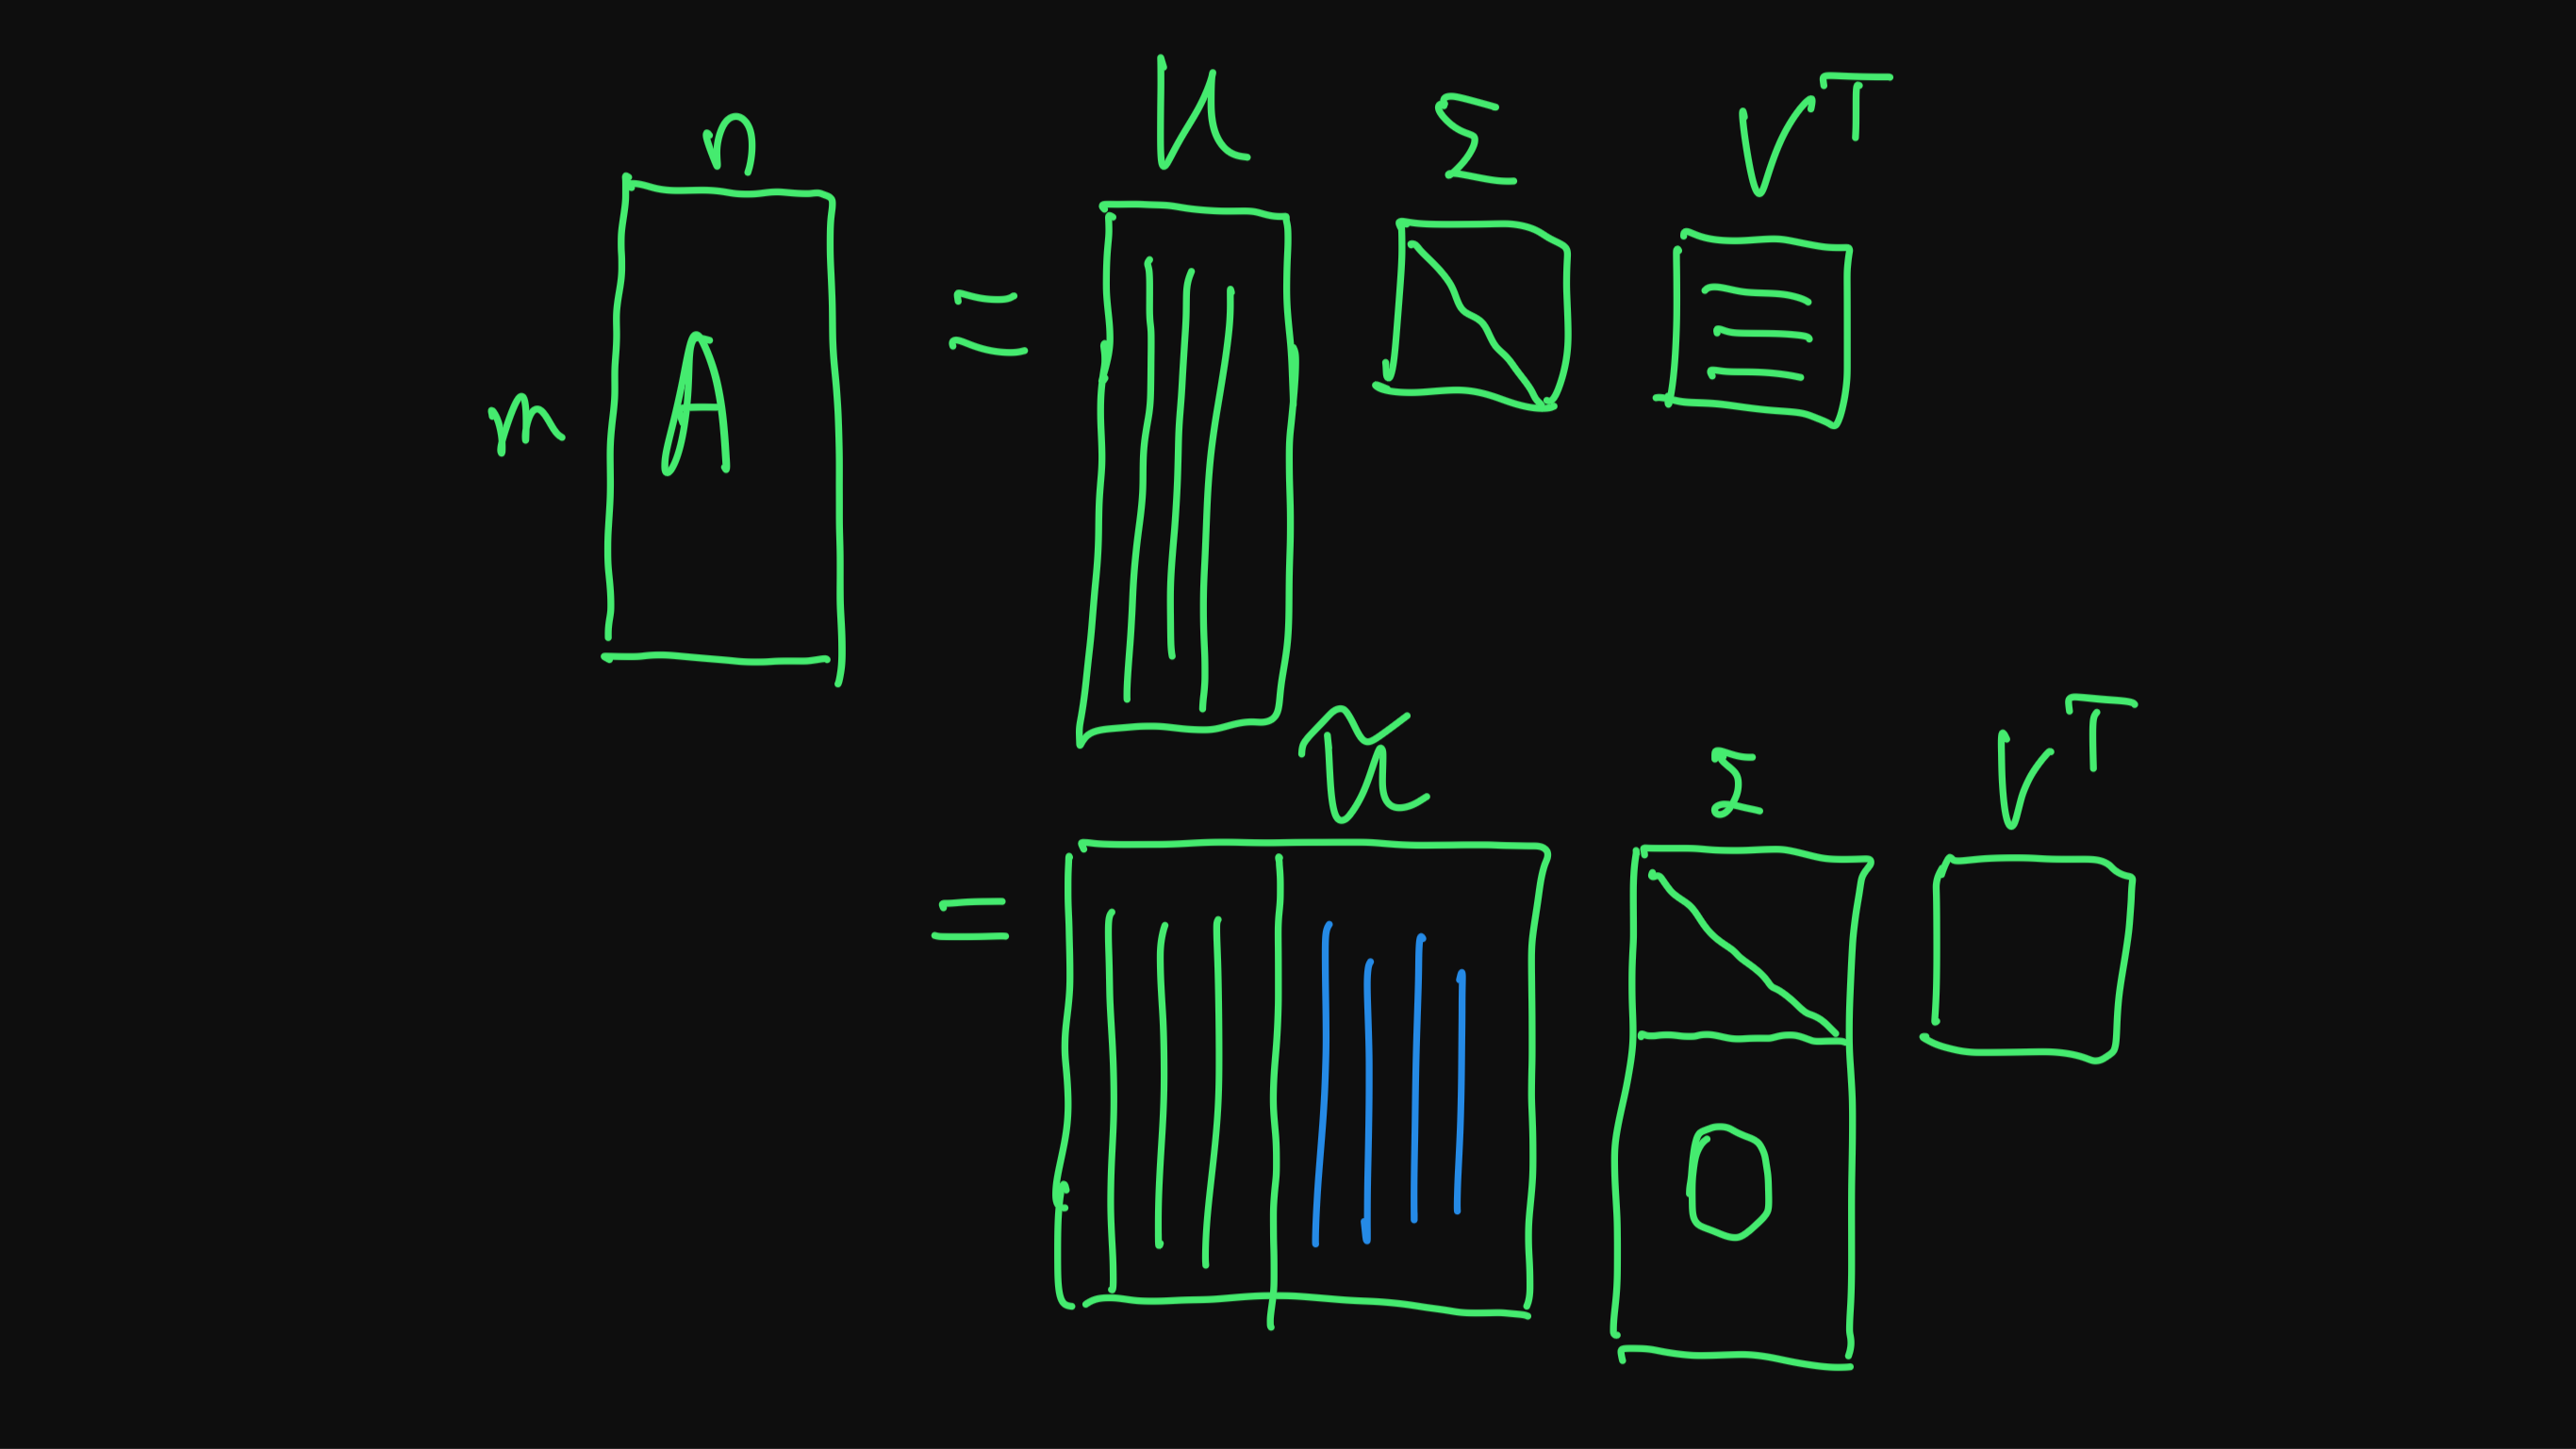
\includegraphics[scale=0.1]{./figures/Thm6-5-4/Full-SVD-Tall.png}}
    \only<2>{
    Full Singular Value Decomposition
    \bigskip

    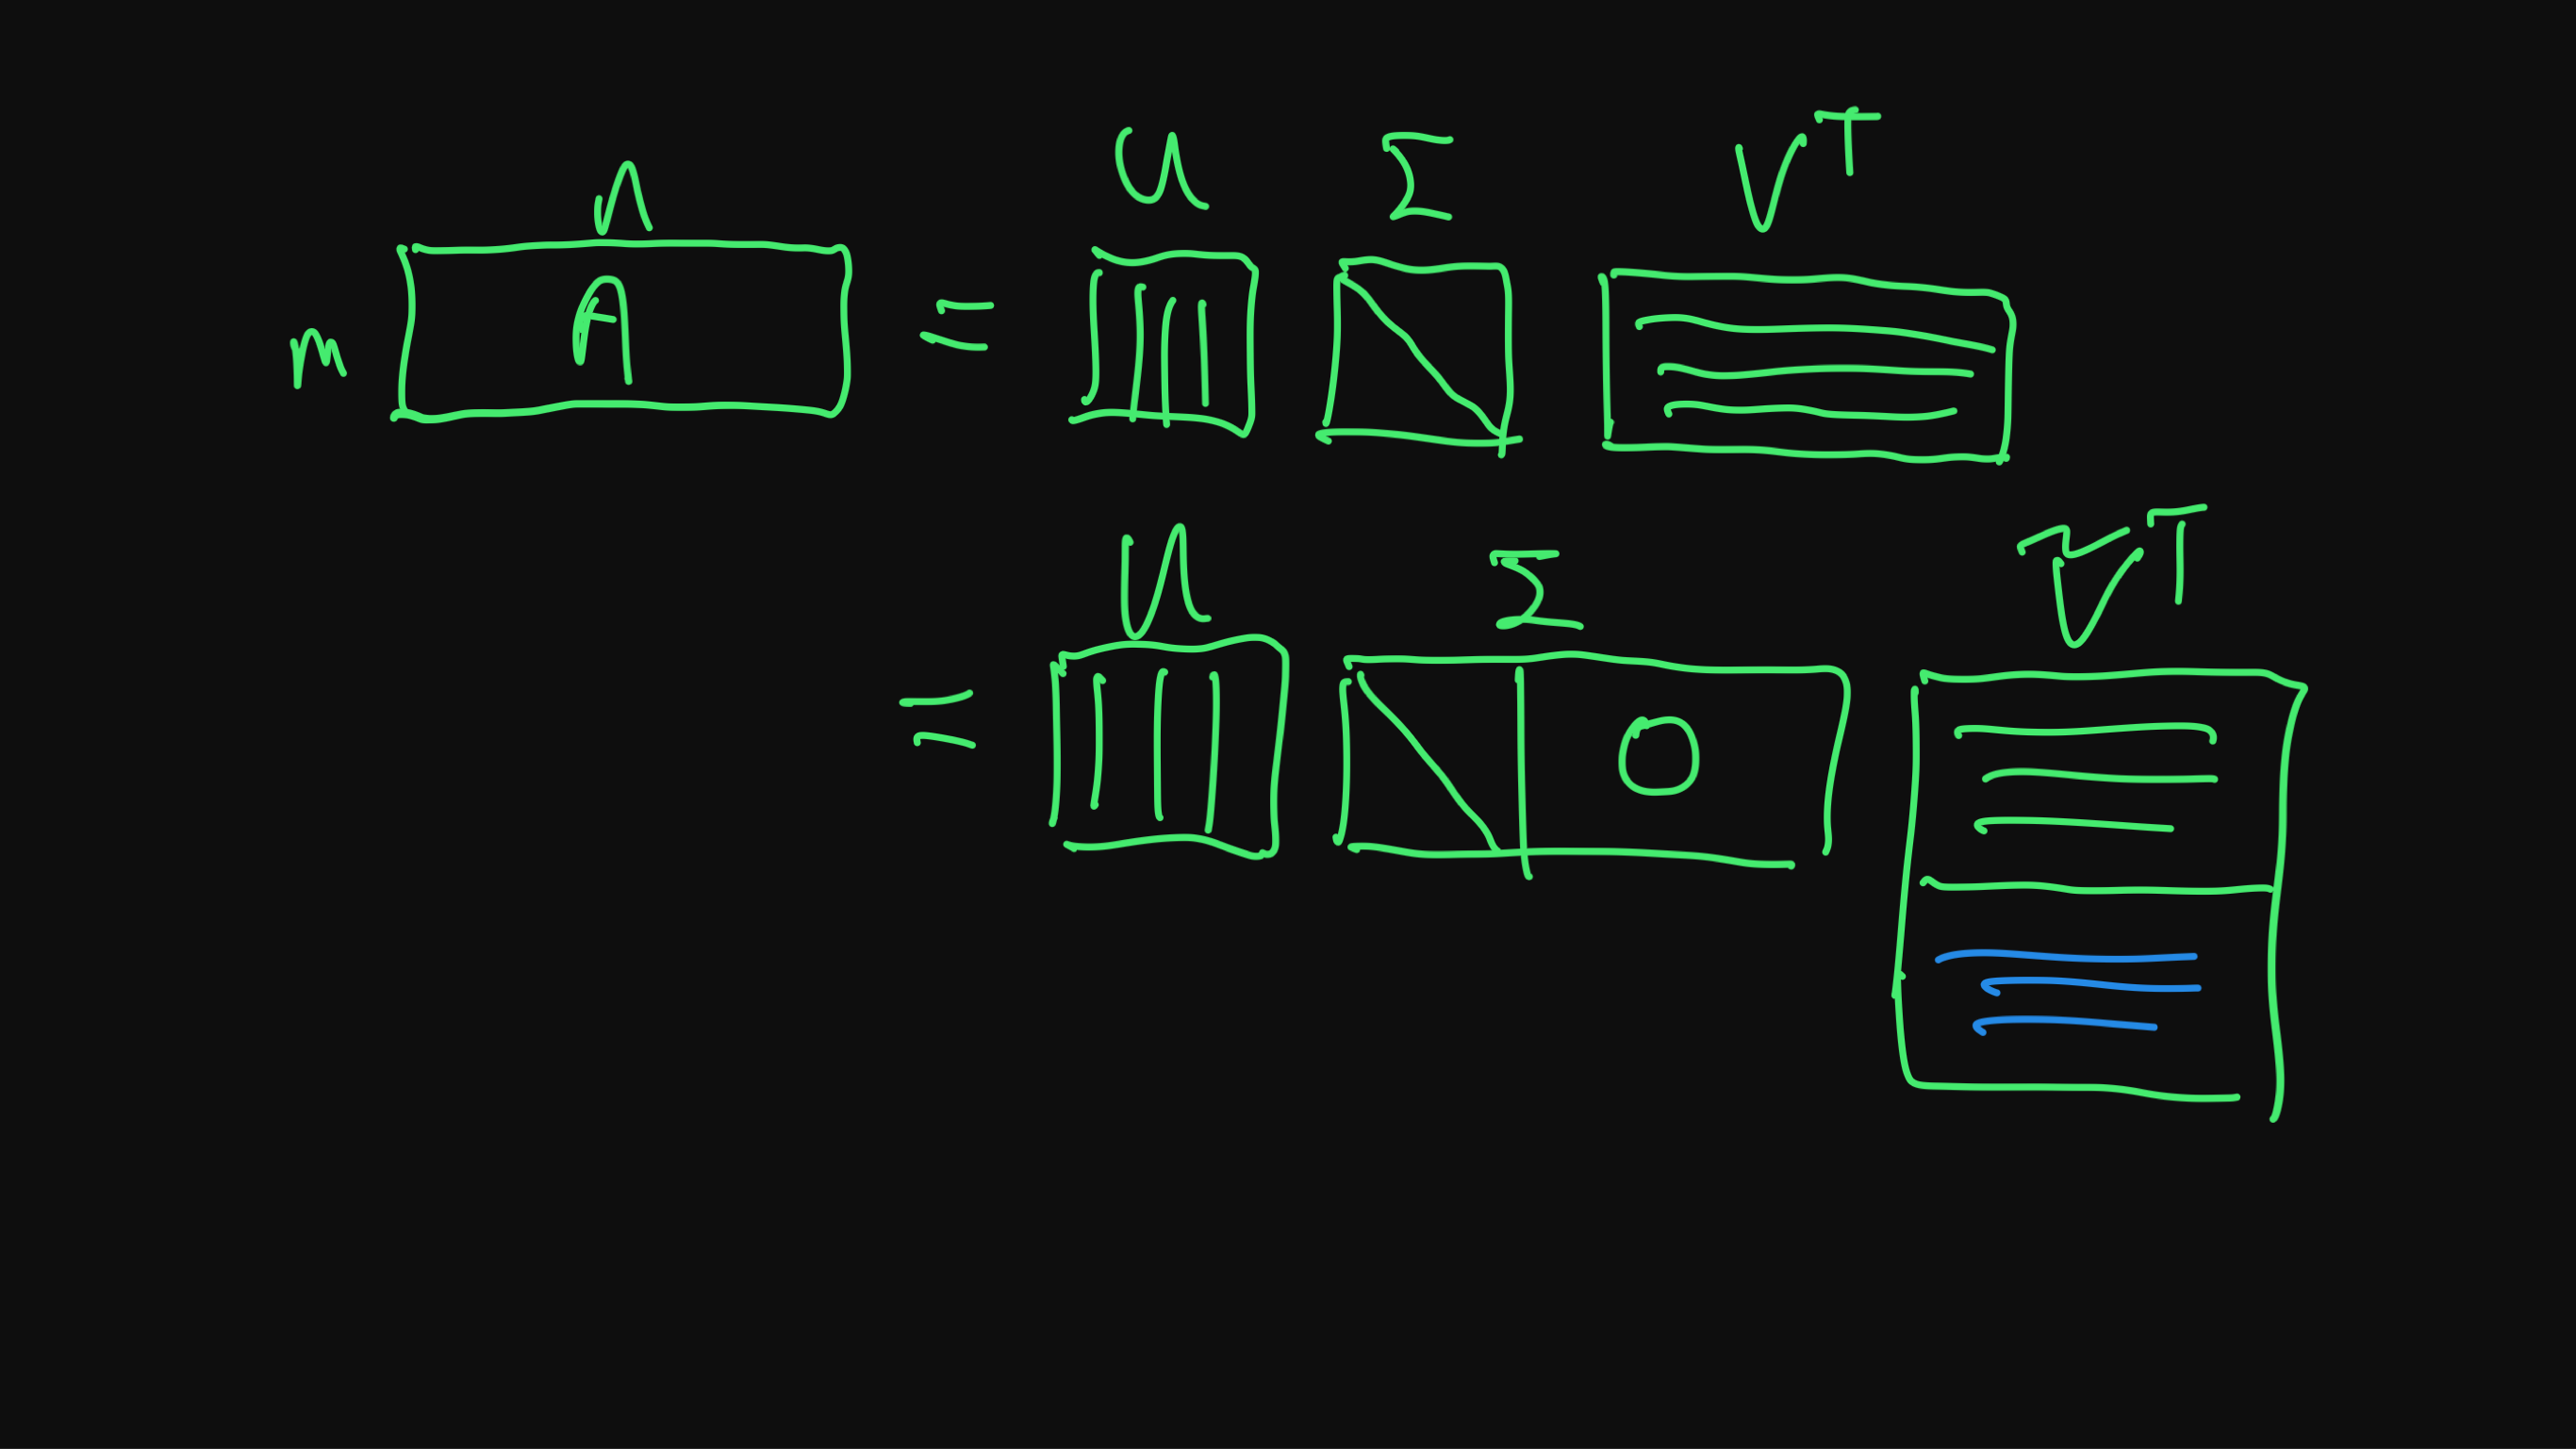
\includegraphics[scale=0.1]{./figures/Thm6-5-4/Full-SVD-Fat.png}}
    \only<3>{\includegraphics[scale=0.035]{./figures/Thm6-5-4/SVD-Spaces.png}}
\end{center}
}
%-------------- end slide -------------------------------%}}}
\section[\textcolor{yellow}{}]{\textcolor{yellow}{Applications}}
%-------------- start slide -----------------------------% {{{ 19
\frame{
\frametitle{Applications}
\pause
\begin{example}[Polar Decomposition]
    \[
	a+bi = \underbrace{\sqrt{a^2+b^2}}_{\text{\textcolor{yellow}{radius}} }\: \underbrace{e^{i\theta}}_{\text{\textcolor{pink}{rotation}} }.
    \]
    Similarly, any square matrix
    \[
	A = U\Sigma V^T  = \underbrace{U \Sigma
	U^T}_{\text{\textcolor{yellow}{nonneg. def.}} } \underbrace{UV^T}_{\text{\textcolor{pink}{rotation}} }
    \]
\end{example}
\vfill
\begin{definition}
    A real $n\times n$ matrix $G$ is \alert{nonnegative definite} (or \alert{positive} in the book) if it is symmetric and for all $\vec{x}\in\R^n $
    \begin{align*}
    	\vec{x}^T G \vec{x}\ge 0.
    \end{align*}
\end{definition}
}
%-------------- end slide -------------------------------%}}}
%-------------- start slide -----------------------------% {{{{ 20
\frame{
\begin{example}[Generalized inverse]
    \begin{center}
	\only<1>{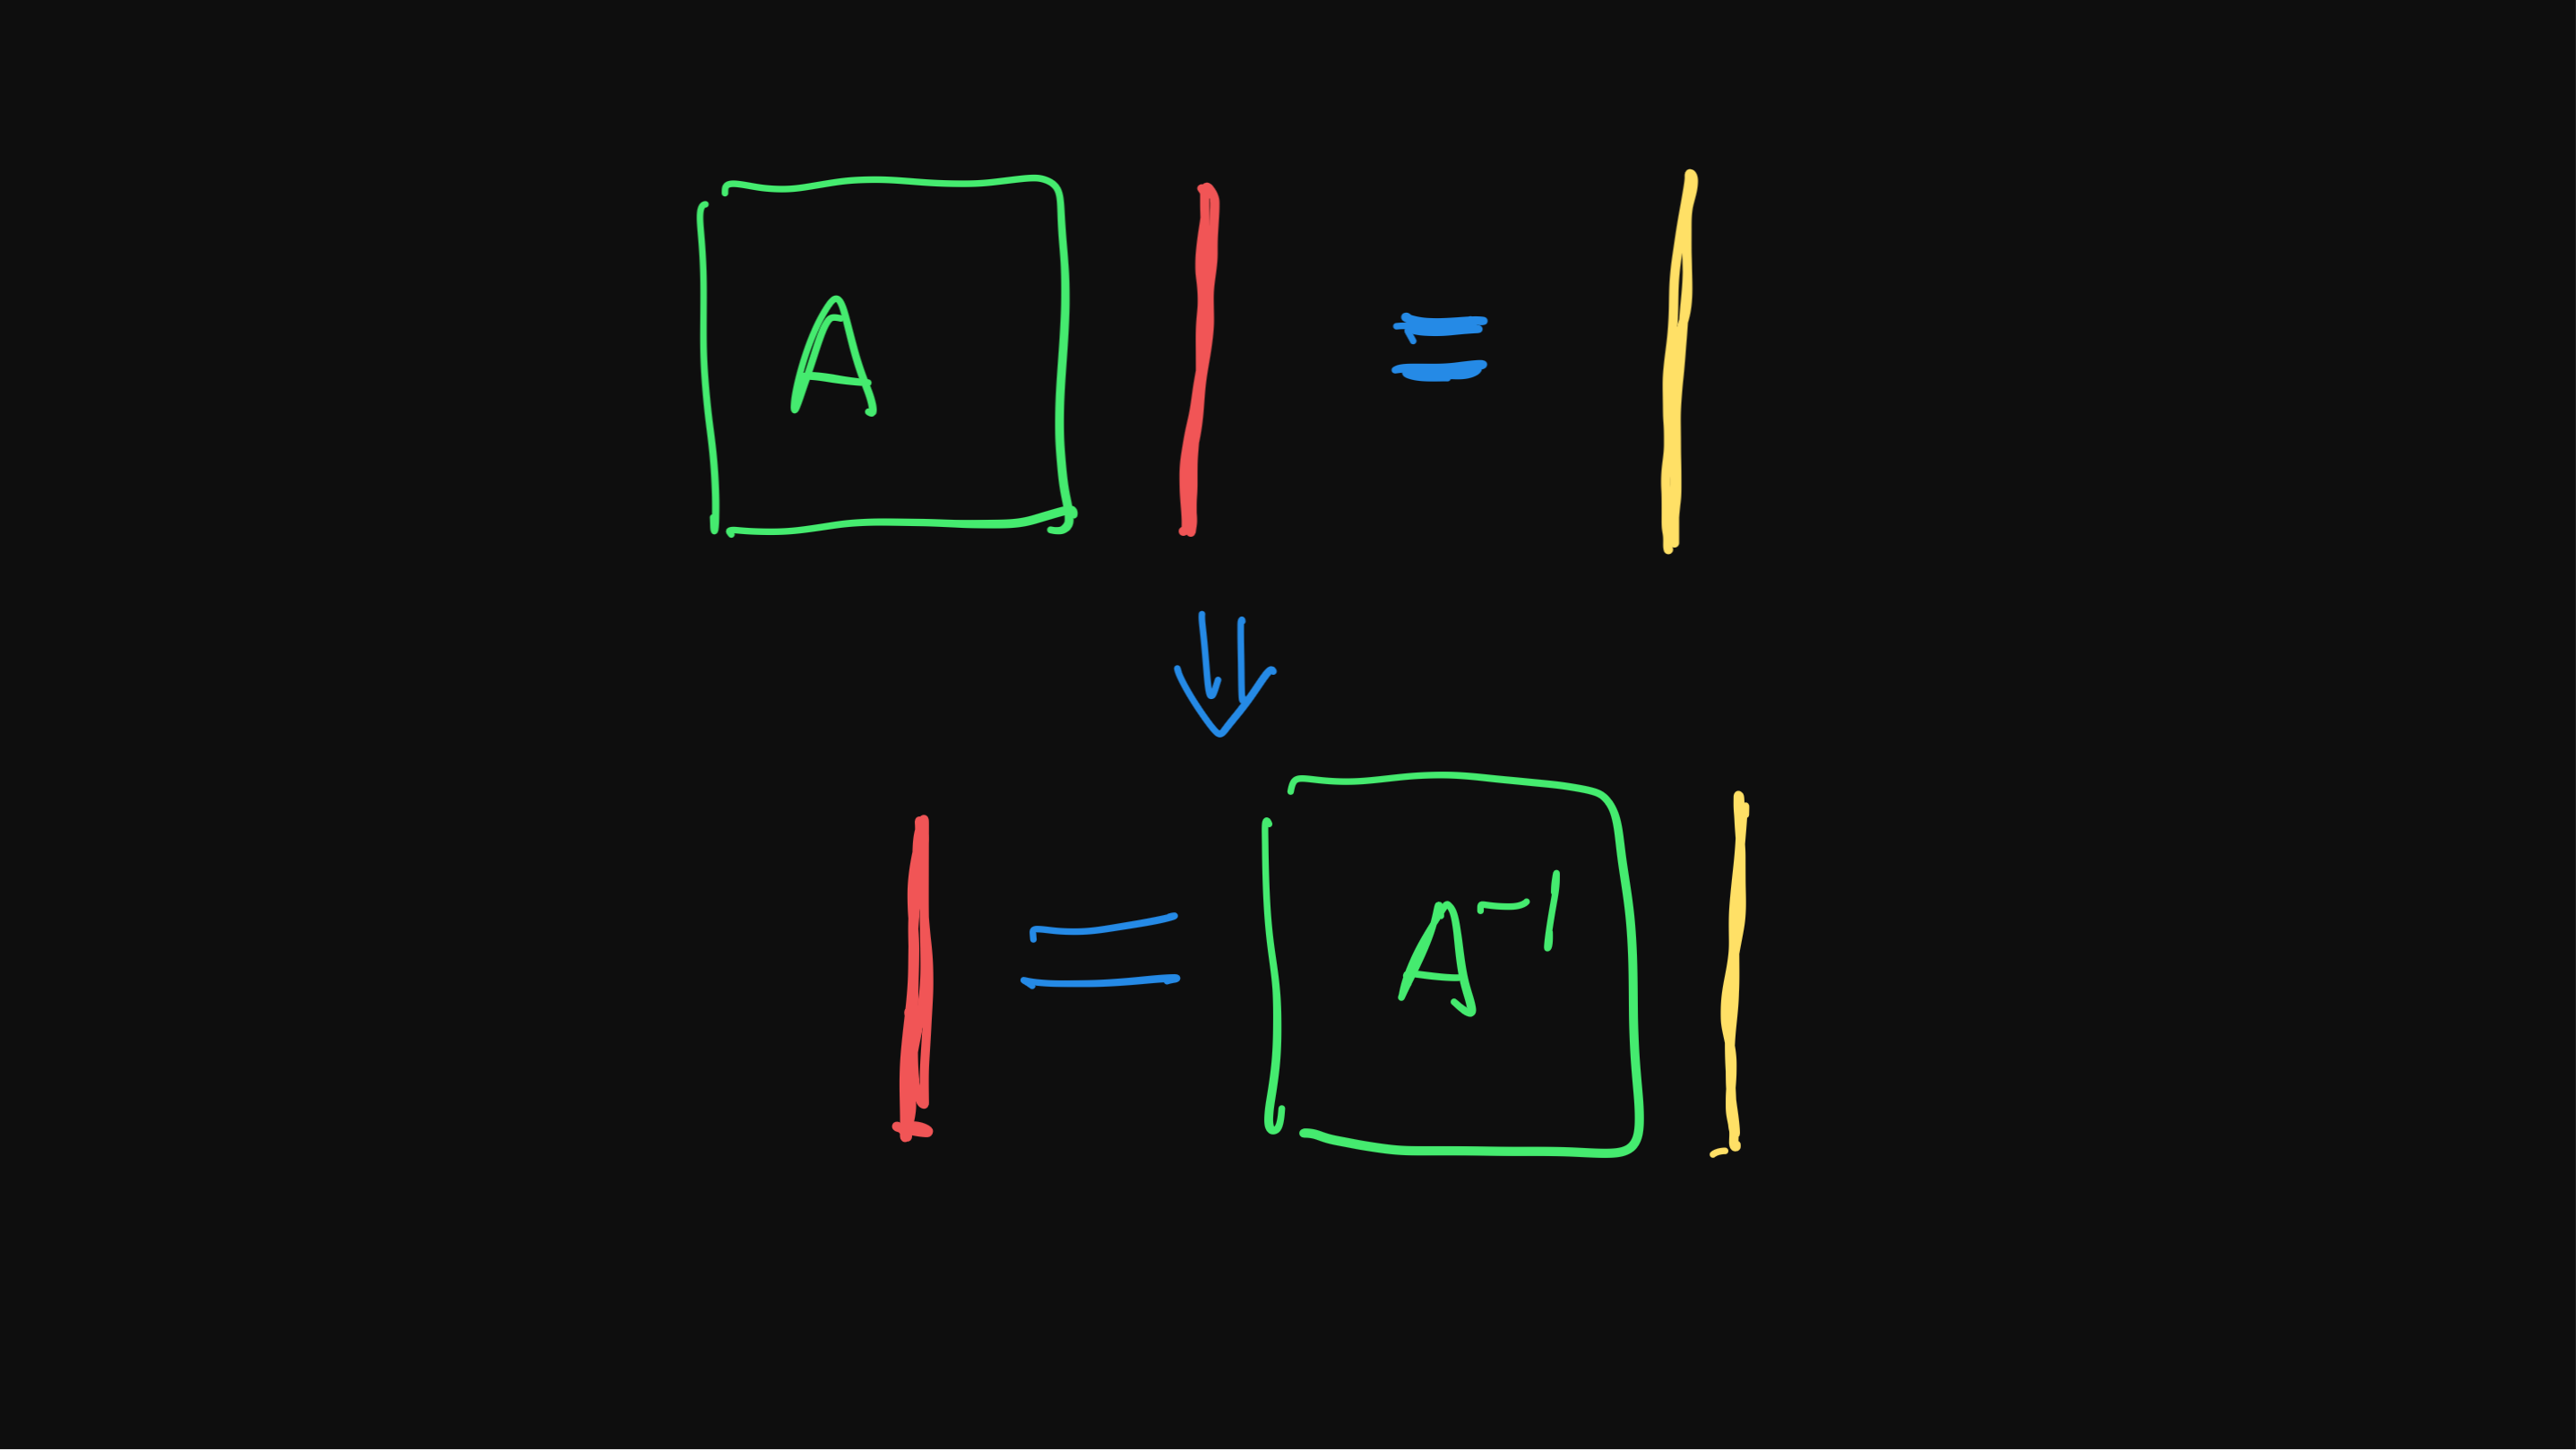
\includegraphics[scale=0.1]{./figures/Thm6-5-4/GInv1.png}}
	\only<2>{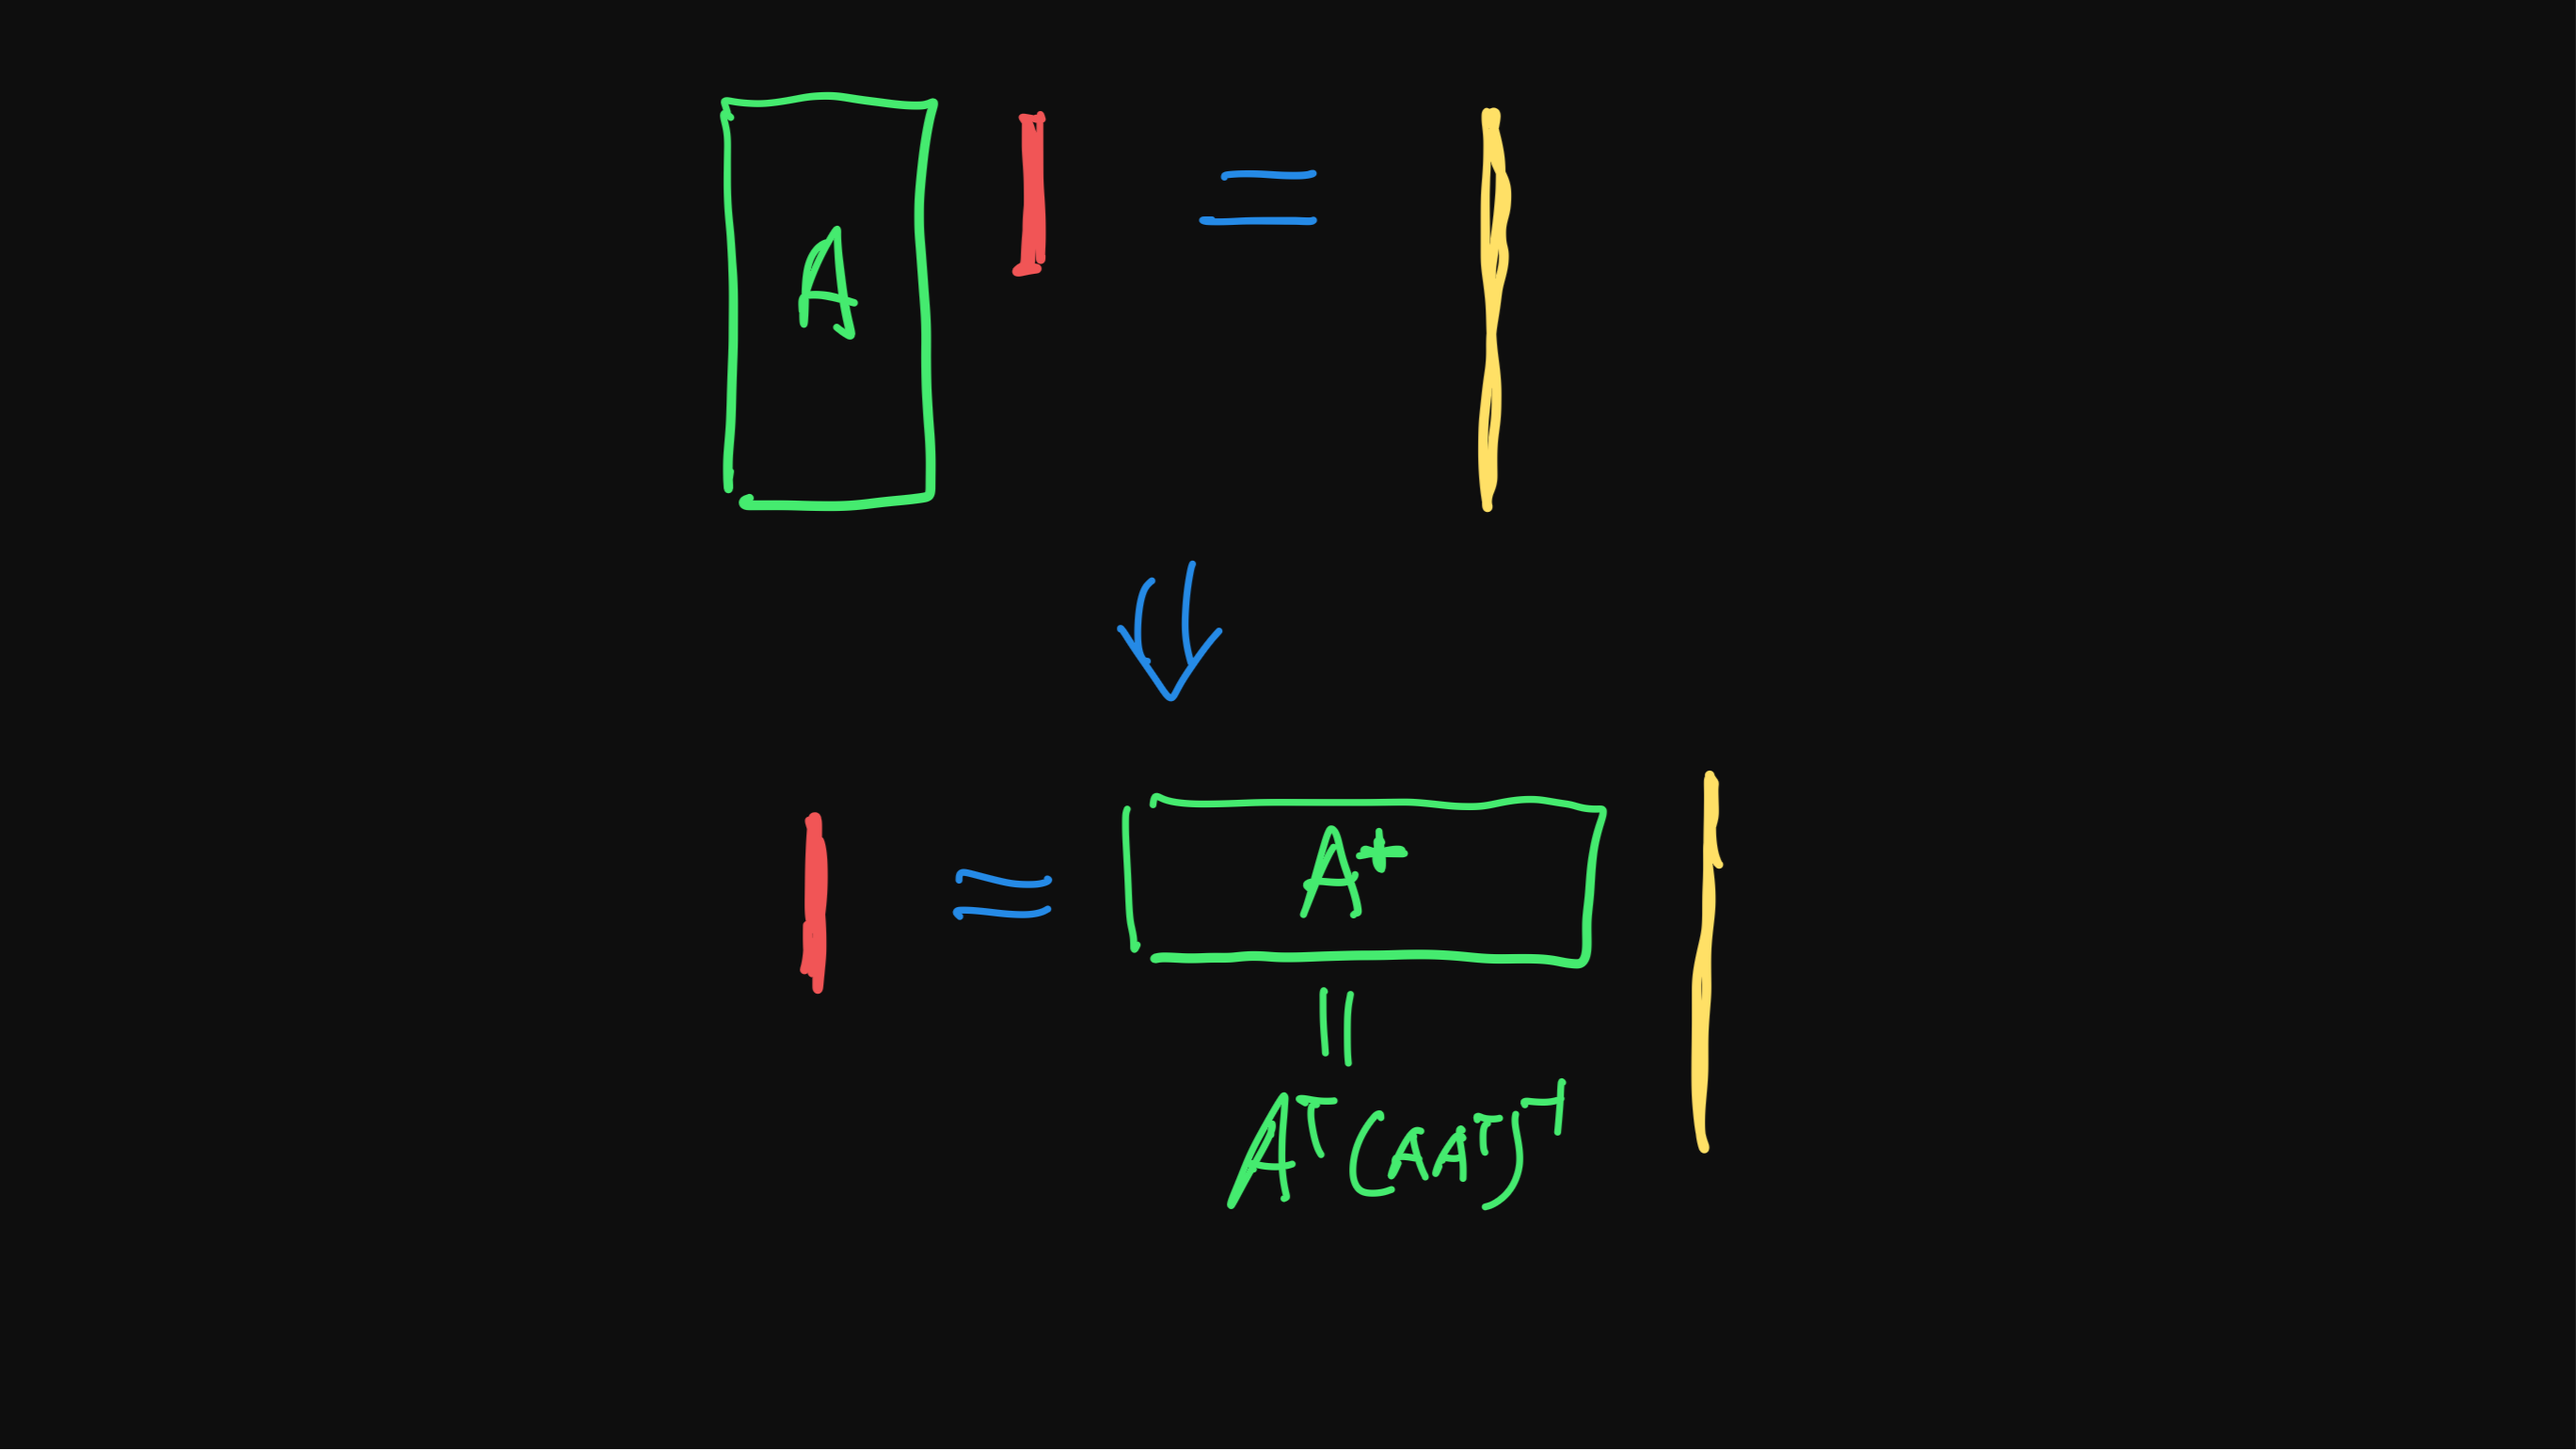
\includegraphics[scale=0.1]{./figures/Thm6-5-4/GInv2.png}}
	\only<3>{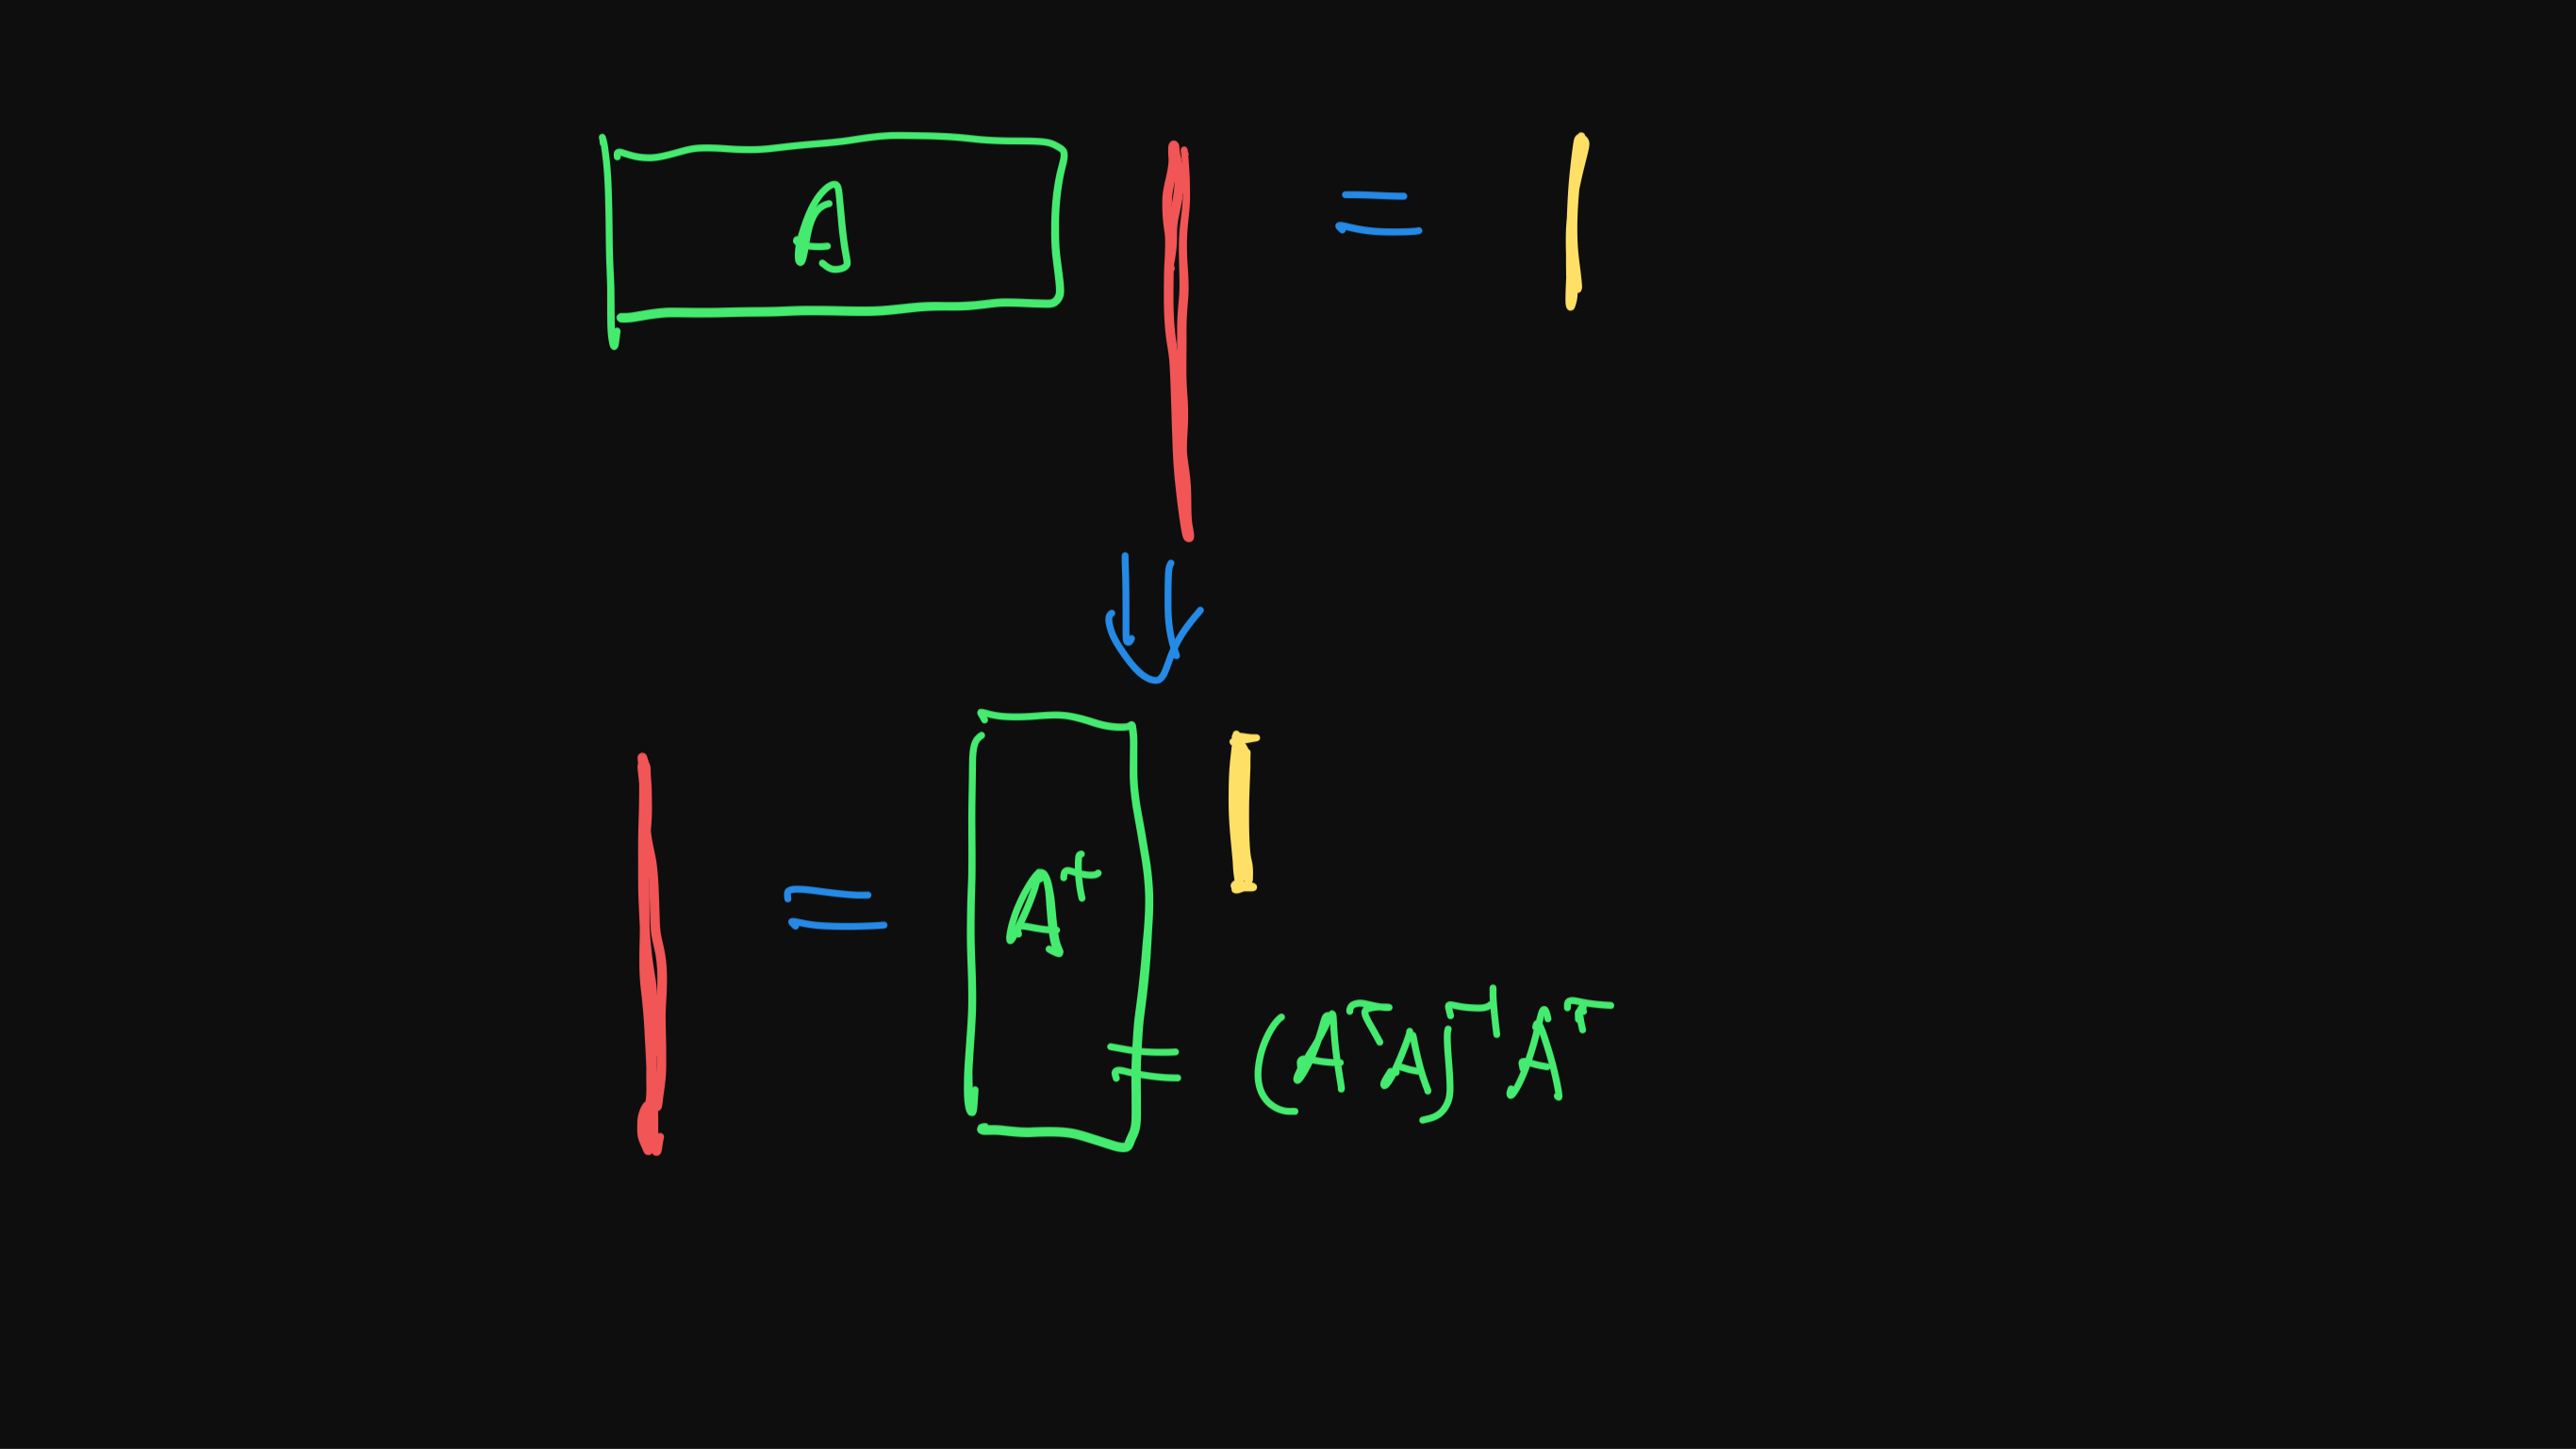
\includegraphics[scale=0.1]{./figures/Thm6-5-4/GInv3.png}}
    \end{center}
\end{example}
}
%-------------- end slide -------------------------------%}}}
%-------------- start slide -----------------------------% {{{{ 21
\frame{
\begin{example}[Image of unit ball under linear transform $A$]
    Let $A=U\Sigma V^T$ be the full SVD for an $m\times n$ matrix $A$. We will see how the unit ball will be mapped:
    \begin{align*}
        \left\{A \vec{x} \mid ||\vec{x}||\le 1 \right\}
    \end{align*}
    \pause
    The linear map $\vec{y}=A \vec{x}$ is trying to do the following things:
    \begin{enumerate}
	\item Rotate the $n$-vector $\vec{x}$ by $V^T$
	\item Stretch along axes by $\sigma_i$ with $\sigma_i=0$ for $i>\rank(A)$
	\item Zero-pad for tall matrix (i.e., $m>n$) or truncate for fat matrix (i.e., $m<n>$) to get $m$-vector
	\item Rotate the $m$-vector by $U^T$
    \end{enumerate}
\end{example}
}
%-------------- end slide -------------------------------%}}}
%-------------- start slide -----------------------------% {{{{ 22
\frame{
\begin{example}[Image of unit ball under linear transform $A$ -- continued]
    \begin{center}
	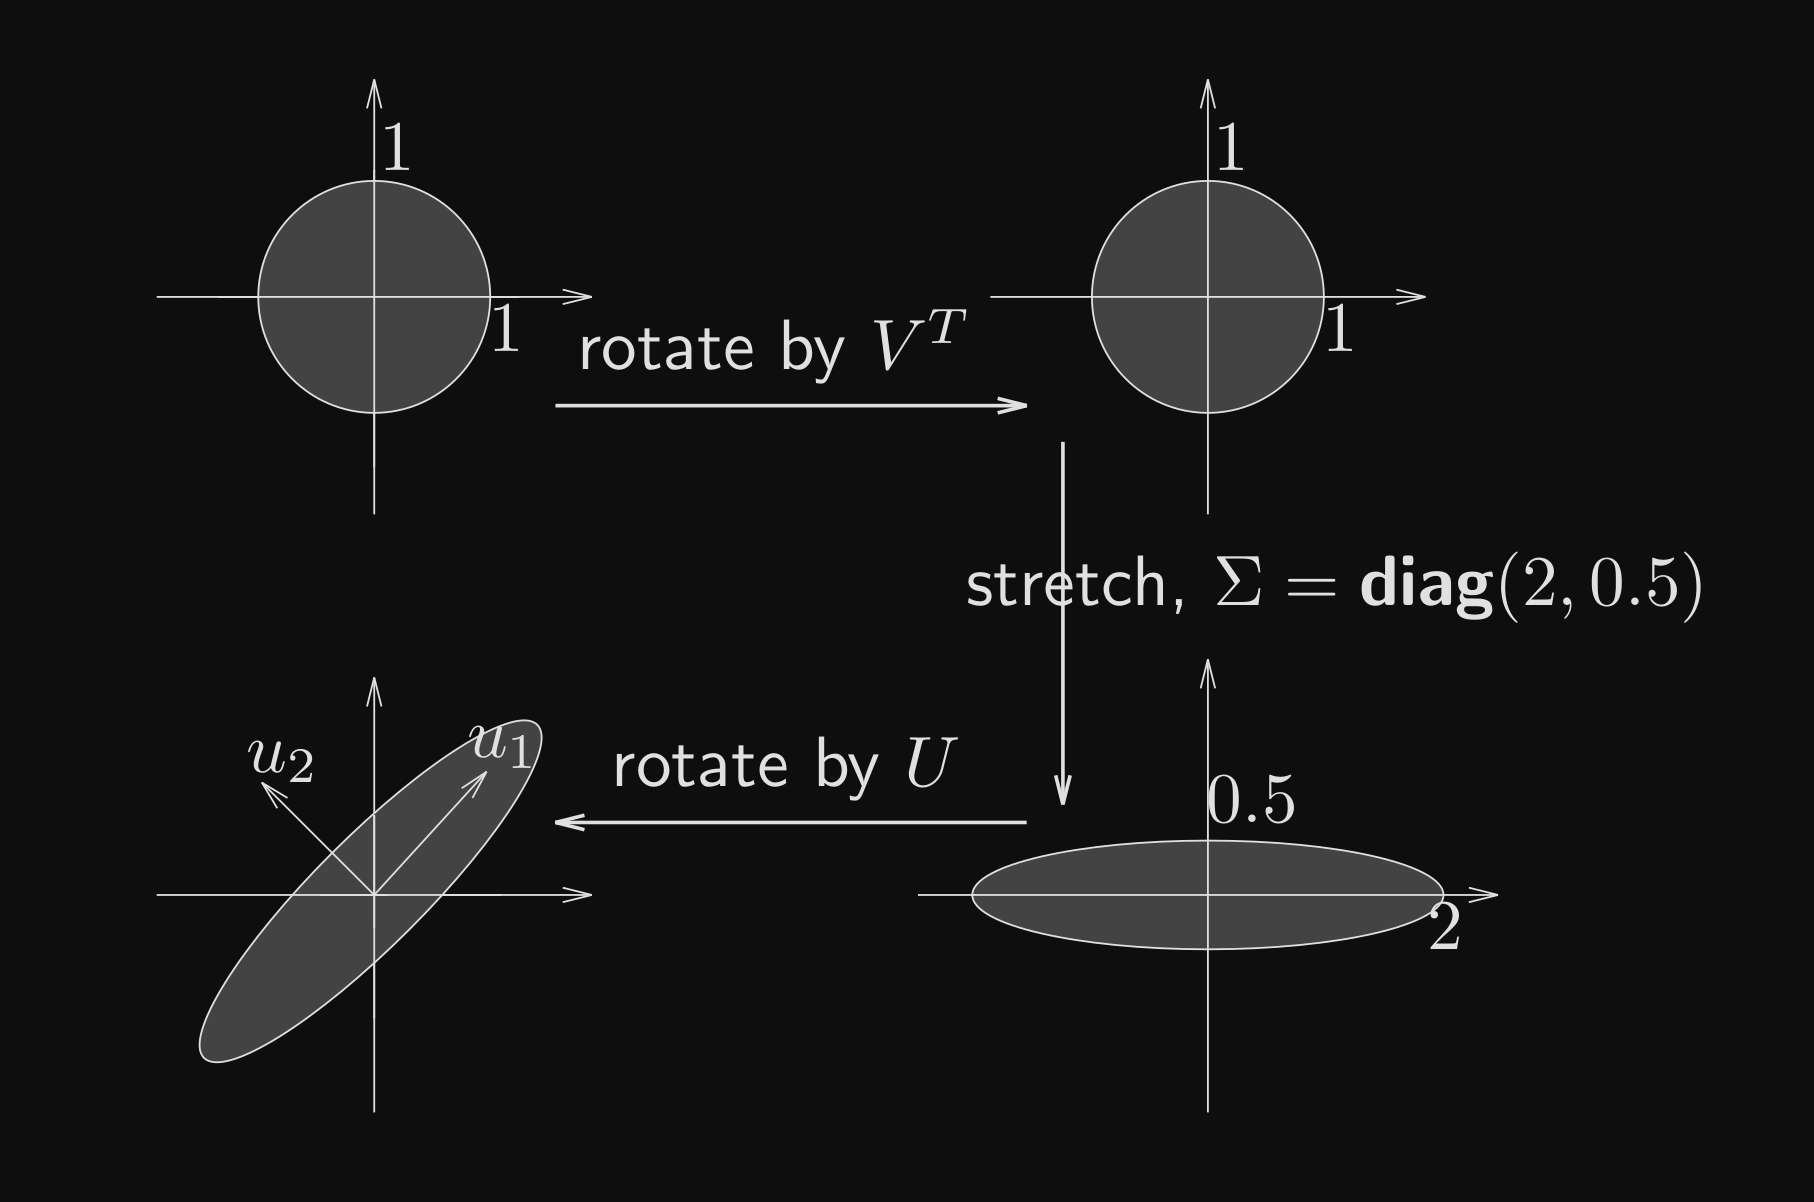
\includegraphics[scale=0.1]{./figures/SVD-Unit-ball.png}
    \end{center}
\end{example}
}
%-------------- end slide -------------------------------%}}}
%-------------- start slide -----------------------------% {{{{ 23
\frame{
\begin{example}[Image Compression]
    \begin{center}
	\only<1>{
	    
\includegraphics[scale=0.3]{./codes/Linear-Algebra-Cartoon-neg.png}

	    Image is a $A$ is a $300\times 300$ matrix.

	    \[
		A\approx \sum_{i=1}^n \sigma_i \vec{u}_i \vec{v}_i^T
	    \]
	}
	\only<2>{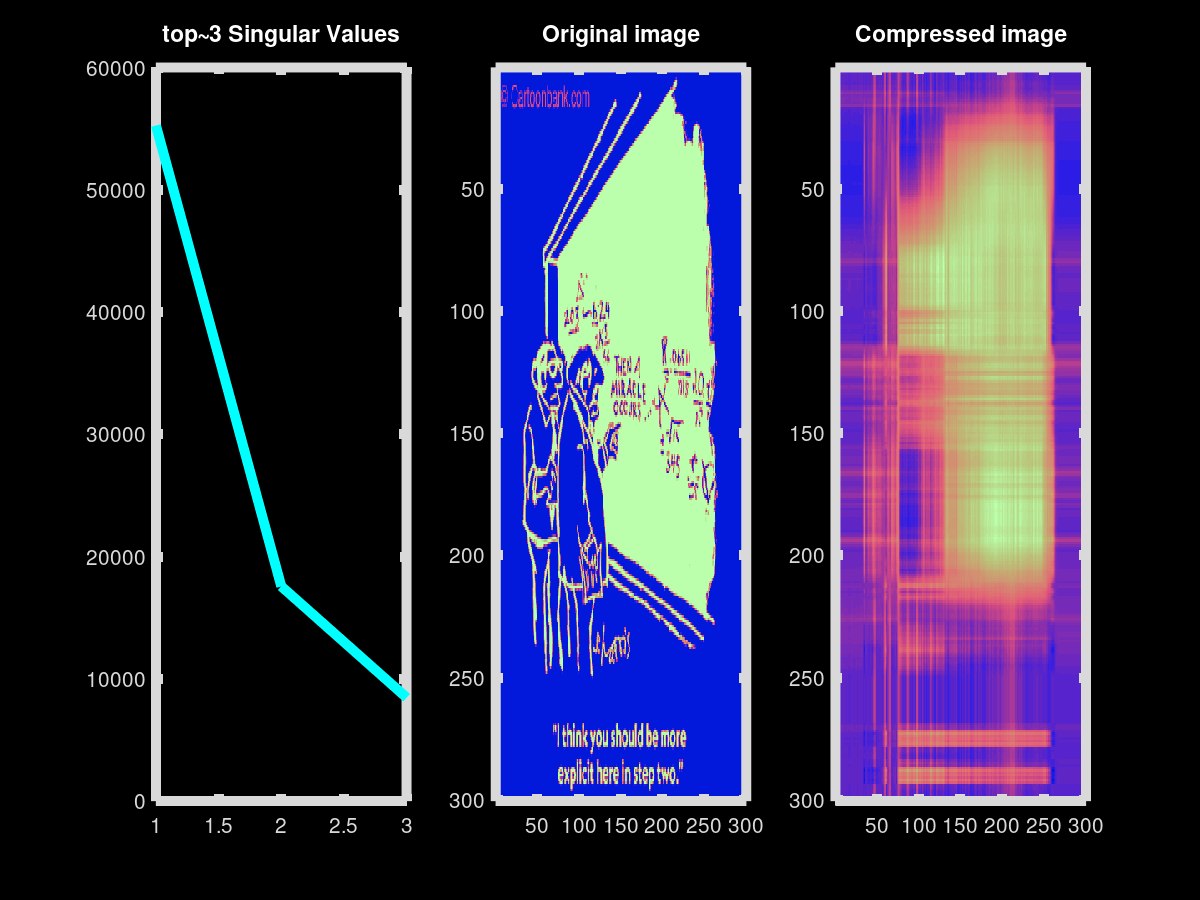
\includegraphics[scale=0.2]{./codes/Svd-ImageCompression-top3-neg.png}}
	\only<3>{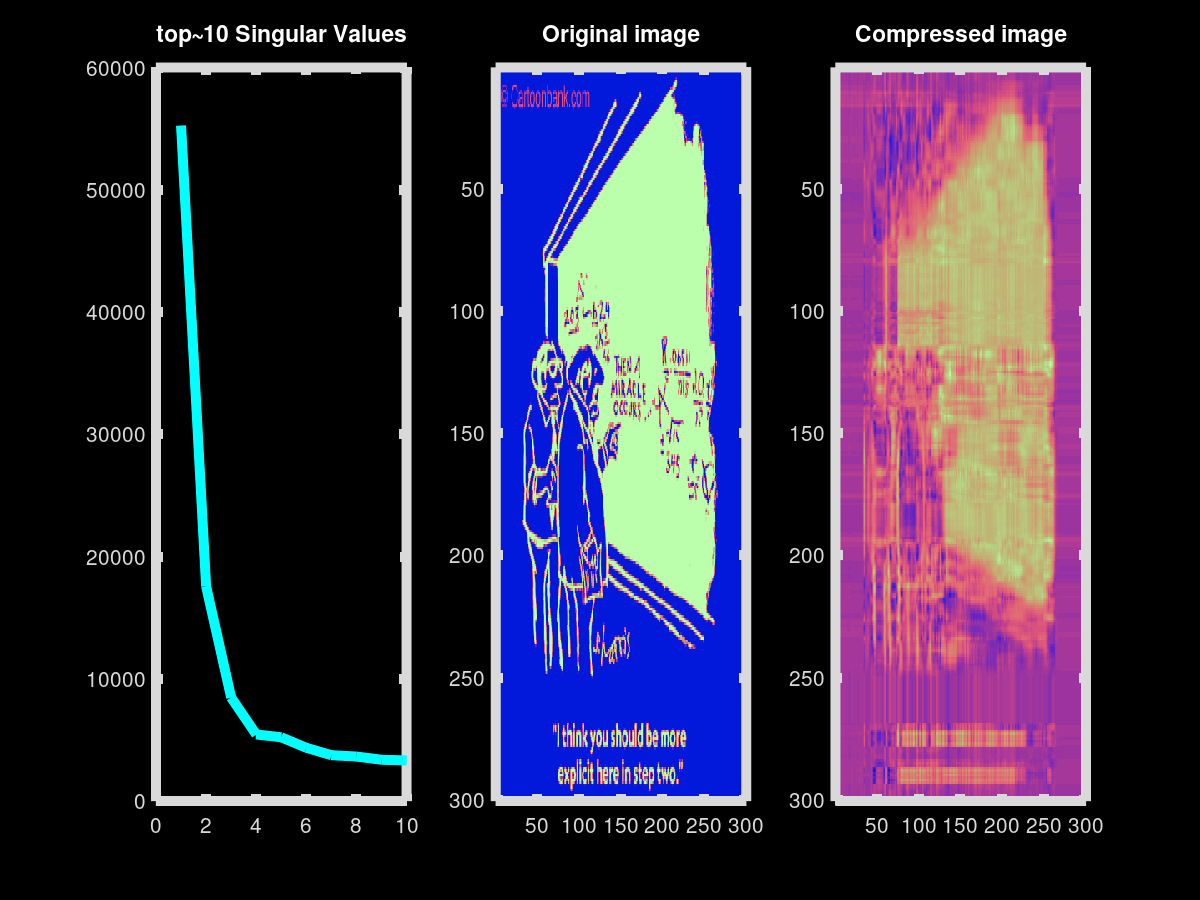
\includegraphics[scale=0.2]{./codes/Svd-ImageCompression-top10-neg.png}}
	\only<4>{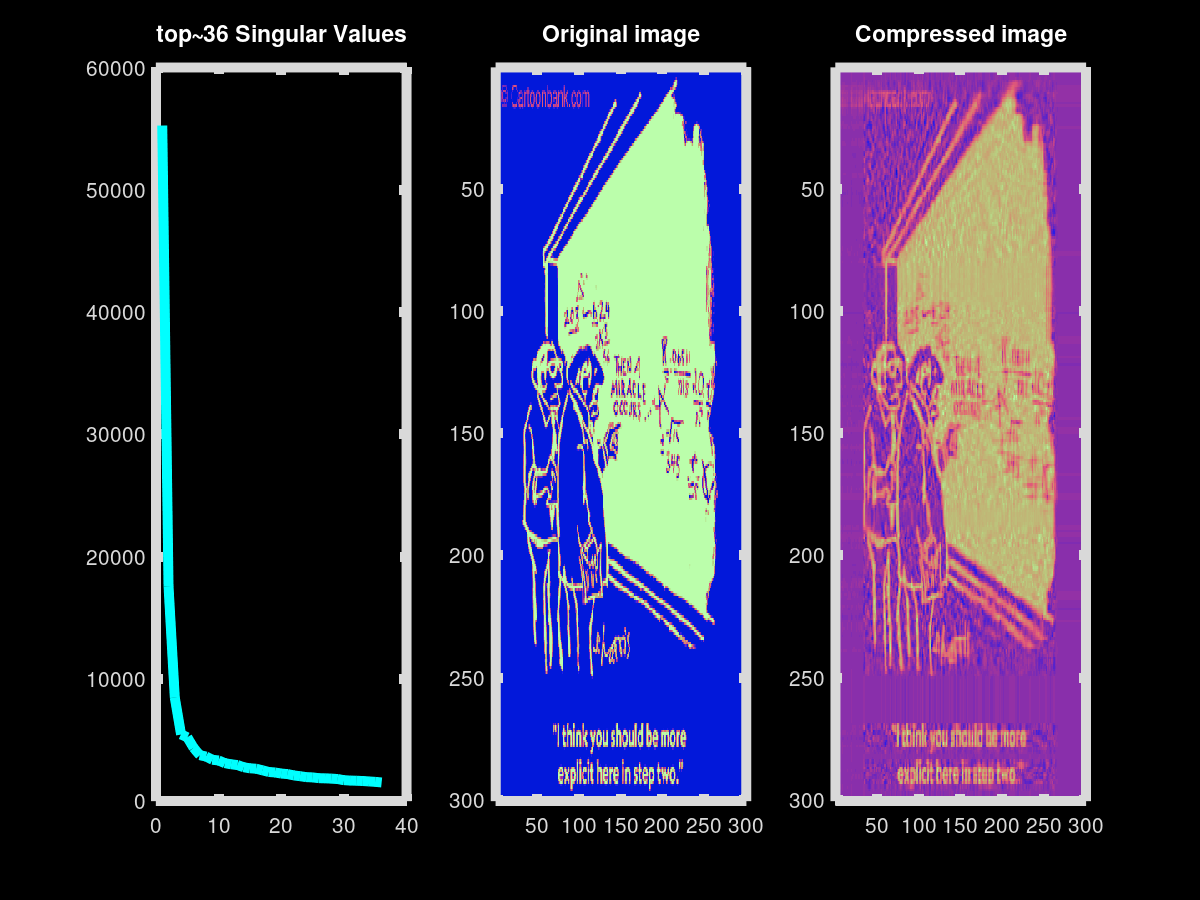
\includegraphics[scale=0.2]{./codes/Svd-ImageCompression-top36-neg.png}}
	\only<5>{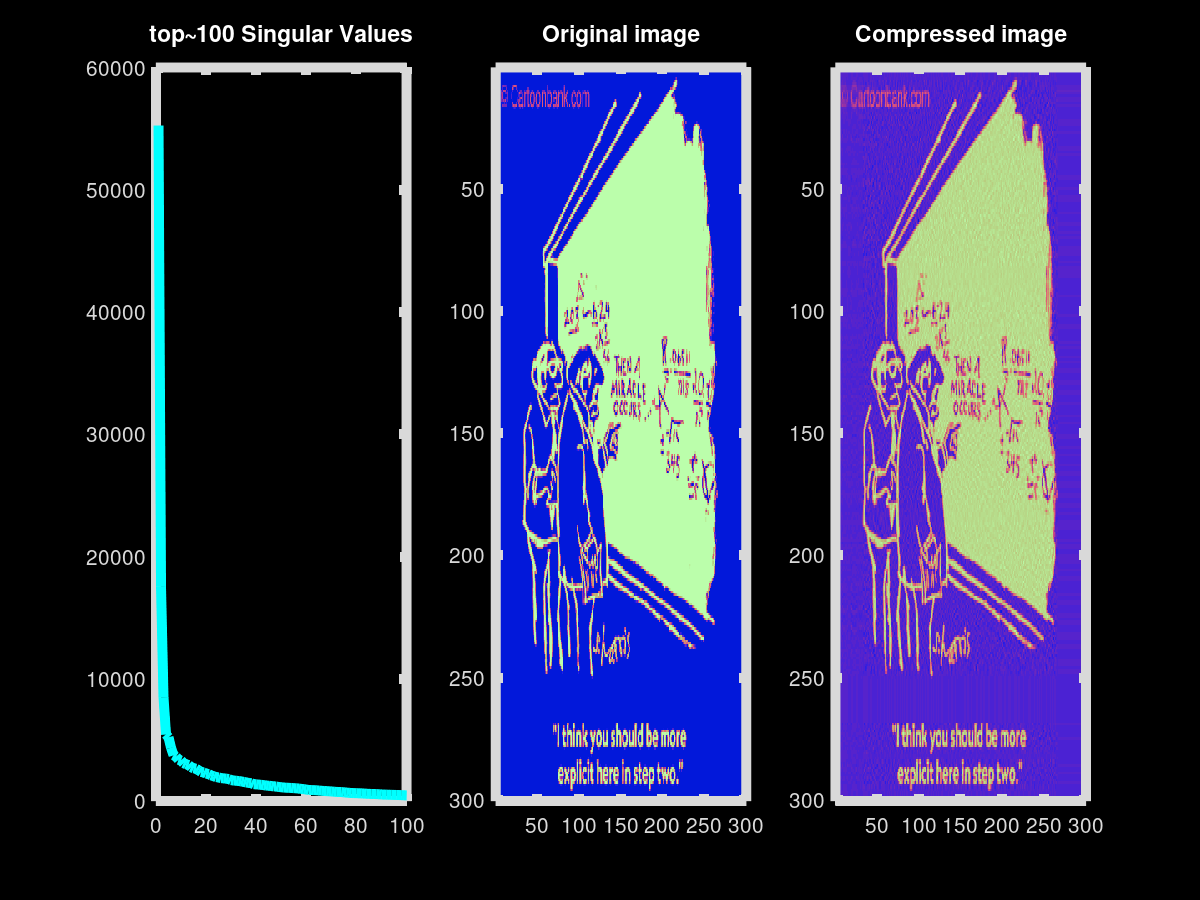
\includegraphics[scale=0.2]{./codes/Svd-ImageCompression-top100-neg.png}}
    \end{center}
\end{example}
}
%-------------- end slide -------------------------------%}}}
\end{document}
